\documentclass[
aip,
jcp,
%preprint,
reprint,
]{revtex4-1}
%
\usepackage[hyperindex,breaklinks,hidelinks,colorlinks,citecolor=blue]{hyperref}
\usepackage{amsmath, amsthm, amssymb}    
\usepackage{float}
%
\usepackage{graphicx}
\DeclareGraphicsExtensions{.pdf,.eps,.png}
\graphicspath{{Figures/}}
\usepackage[outdir=Figures/]{epstopdf}
%
\usepackage{natmove}
%
%\usepackage{mathtools}
%\mathtoolsset{showonlyrefs}
%
\DeclareMathOperator\arctanh{arctanh}
\DeclareMathOperator\arcsinh{arcsinh}
\DeclareMathOperator\sech{sech}
%
\newcommand{\mt}[1]{\boldsymbol{\mathbf{#1}}}          % matrix symbol
\newcommand{\vt}[1]{\boldsymbol{\mathbf{#1}}}          % vector symbol
\newcommand{\tr}[1]{#1^\text{t}}                       % transposition
\newcommand{\diff}[2]{\frac{\partial #2}{\partial #1}} % derivative
\newcommand{\avg}[1]{\overline{#1}}                    % average
%\newcommand{\Liu}[1]{\mathcal{L}_{#1}}                 % Liouville operator
\newcommand{\Liu}{\mathcal{L}}
\newcommand{\Ham}[1]{{\mathcal H}_\mathrm{#1}}         % Hamiltonian
\newcommand{\nn}{n}

\begin{document}

\author{Charlles R. A. Abreu}
\email{abreu@eq.ufrj.br}
\affiliation{Chemical Engineering Department, Escola de Qu\'imica, Universidade Federal do Rio de Janeiro, Rio de Janeiro, RJ 21941-909, Brazil}
\affiliation{Department of Chemistry, New York University, New York, New York 10003, USA}

\author{Mark E. Tuckerman}
\email{marktuckerman@nyu.edu}
\affiliation{Department of Chemistry, New York University, New York, New York 10003, USA}
\affiliation{Courant Institute of Mathematical Sciences, New York University, New York, New York 10012, USA}
\affiliation{NYU-ECNU Center for Computational Chemistry at NYU Shanghai, Shanghai 200062, China}

\title{A Simple Principle Behind the Isokinetic Strategy for Resonance Control in Multiple Time-Scale Molecular Dynamics}

\keywords{molecular dynamics; multiple time-stepping; resonance}

\date{\today}

\maketitle

\section{Introduction}

Multiple time-scale (MTS) integration \cite{Grubmuller_1991, Tuckerman_1992, Martyna_1996} is an effective way of improving the efficiency of Molecular Dynamics (MD) simulations.
In classical MD, it allows the most expensive computations, such as the evaluation of long-range van der Waals and electrostatic components of force fields, to be done less frequently than others.
This is possible because the time scale of variations in such contributions is much larger than those in both short-ranged non-bonded interactions and bonded intramolecular forces.
If estimating ensemble averages is the main goal of a simulation, then the maximum benefit one can get from multiple time-stepping occurs when it is possible to match the longest-scale step size with the correlation time of the system dynamics, i.e., the sampling period required to obtain a series of uncorrelated configurations.
Although this is theoretically feasible in many situations, it took long until the capacity of the MTS strategy could be fully realized.
The cause of this delay is the existence of resonance artifacts \cite{Biesiadecki_1993, Schlick_1998, Ma_2003} that constrain the maximum attainable step size.
Attempts have been made over the years to overcome this limitation.
One of the strategies, known as mollified impulse \cite{Garcia-archilla_1998, Griebel_1999}, relies on altering the slow part of the potential energy function.
This is done by evaluating the corresponding forces at filtered positions, averaged along auxiliary trajectories which are, in turn, dictated by the fast part of the potential.

The most successful approach for dealing with resonance artifacts in thermostatted MD does not involve altering the potential.
Instead, it entails introducing new dynamic variables (extended system approach) and enforcing isokinetic constraints \cite{Minary_2003, Minary_2003_2, Minary_2004, Leimkuhler_2013}.
The basic recipe consists in pairing an extra velocity with the actual velocity of each degree of freedom in the system.
Then, independent thermostats are attached to all extra velocities.
However, instead of letting them vary without bounds, the combined kinetic energy of each velocity pair is enforced to be constant.
In this way, the magnitude of every actual velocity can never exceed a certain value, thus avoiding resonance and instability in the simulated dynamics.
This procedure is clearly not meant to reproduce the Maxwell-Boltzmann distribution of velocities of a canonical ensemble, but it provably provides the correct distribution of coordinates \cite{Minary_2003, Minary_2003_2, Minary_2004, Leimkuhler_2013}.
In a more elaborate version, several extra velocities (with their attached thermostats) are associated to each degree of freedom and take part in the isokinetic constraints.
The method was originally formulated \cite{Minary_2003, Minary_2003_2, Minary_2004} with deterministic thermostats \cite{Martyna_1992} and subsequently reformulated \cite{Leimkuhler_2013} with stochastic ones \cite{Samoletov_2007, Leimkuhler_2009}.

There is a rich literature on the development and analysis of extended-system methods \cite{Martyna_1996, Tuckerman_1999, Tuckerman_2001, Sergi_2001, Ezra_2004, Tuckerman_2010}.
Pioneered in the 1980's \cite{Andersen_1980, Nose_1984, Hoover_1985}, they allowed the use of MD to study thermodynamic systems under the influence of external baths.
Nevertheless, the isokinetic formulation is somewhat extraneous in such universe.
Some of the well-established tools developed in the area are not readily applicable to its analysis.
As a consequence, knowledge about the properties of isokinetic methods has been advancing in a case-by-case basis.
Once this is the first approach that allows MTS simulations with very large time steps, it becomes particularly hard to distinguish the actual cause of observed anomalies.

In the present paper, we introduce a novel resonance-control methodology and demonstrate that it is completely equivalent to the isokinetic framework.
It consists in substituting the kinetic part of the system Hamiltonian by a new momentum-dependent function, whose main feature is also causing the confinement of velocities to a fixed range.
The potential part of the Hamiltonian is kept unchanged.
We are, thus, recasting the isokinetic approach is a form that is more akin to standard extended-system and stochastic methods.
This allowed us to unveil certain properties of the isokinetic dynamics which remained hitherto unnoticed, such as 1) the driven-variable nature of the extra velocities, 2) the existence of additional conserved quantities, and 3) some odd forms of velocity frequency distributions.
More importantly, it became straightforward to devise a new, Langevin-type version of the method with superior performance.

\section{Methods}

\subsection{Speed-Limiting Hamiltonian for Isothermal Dynamics}

For a classical system with coordinates $\vt r$, we are often interested in obtaining canonical averages of a purely configurational property, say,
\begin{equation}
\label{eq:configurational average}
\langle A \rangle = \frac{1}{Z} \int e^{-\frac{U(\vt r)}{kT}} A(\vt r) d\vt r,
\end{equation}
where $T$ is temperature, $k$ is the Boltzmann constant, $U(\vt r)$ is a potential energy function, and $Z$ is a normalizing constant.
This is usually accomplished by defining a Hamiltonian $\mathcal{H}(\vt r, \vt p) = U(\vt r) + \sum_{i=1}^{N_f} \frac{p_i^2}{2 m_i}$ and exploring the phase space by means of some NVT dynamics method.
In this expression, $\vt p$ is the momentum vector and $m_i$ is the mass associated to each degree of freedom $i$, whose total number is $N_f$.
This procedure results in a probability density $\rho(\vt r, \vt p) \propto e^{-\frac{\mathcal{H}(\vt r, \vt p)}{kT}}$, up to small systematic deviations introduced by time discretization.
Coordinates are sampled with the desired probabilities and, at the same time, each momentum $p_i$ fluctuates according to a normal distribution with mean $g_i = 0$ and standard deviation $\sigma_i = \sqrt{m_i k T}$, i.e.
\begin{equation}
\label{eq:gaussian momentum distribution}
\rho(p_i) = \frac{1}{\sqrt{2 \pi m_i k T}} e^{-\frac{p_i^2}{2 m_i k T}}.
%\rho(p_i) \propto e^{-\frac{p_i^2}{2 m_i k T}}.
\end{equation}

Nonetheless, the details of the momentum distribution are not particularly relevant if one is only interested in configurational averages.
In this context, we propose the use of a modified Hamiltonian
\begin{equation}
\label{eq:modified hamiltonian}
\mathcal{H}_n(\vt r, \vt p) = U(\vt r) + \nn kT \sum_{i=1}^{N_f} \ln \cosh\left(\frac{p_i}{\sqrt{\nn m_i k T}}\right),
\end{equation}
where $\nn$ is a positive, otherwise arbitrary parameter.
For simplicity, we will only consider integer values.
The standard Hamiltonian is approached by increasing $\nn$, as one can observe in the Taylor series expansion
\begin{equation*}
\nn \ln \cosh \left(\frac{x}{\sqrt{\nn}}\right) = \frac{x^2}{2} - \frac{x^4}{12 \nn} + \frac{x^6}{45 \nn^2} + \mathcal{O}(x^8).
%\nn \ln \cosh \left(\frac{x}{\sqrt{\nn}}\right) = \frac{x^2}{2} \left[1 - \frac{x^2}{6 \nn} + \frac{2 x^4}{45 \nn^2} + \mathcal{O}(x^6) \right].
\end{equation*}

In an NVT simulation with the modified Hamiltonian, coordinates will still be sampled proportionally to $e^{-\frac{U(\vt r)}{kT}}$, but each momentum $p_i$ will be sampled according to the probability density function (PDF)
\begin{equation}
\label{eq:momentum distribution}
\rho_n(p_i) = \frac{\Gamma\left(\frac{\nn+1}{2}\right)}{\Gamma\left(\frac{\nn}{2}\right) \sqrt{\pi \nn m_i k T}} \sech^\nn\left(\frac{p_i}{\sqrt{\nn m_i k T}}\right),
\end{equation}
which can be interpreted as a generalized logistic distribution.
This PDF, whose derivation is given in Appendix \ref{sec:momentum and velocity distributions}, is depicted for various values of $\nn$ in Fig.~\ref{fig:momentum distributions and velocity definition}(a), where the tendency towards the normal distribution is clear.

\begin{figure}
	\centering
	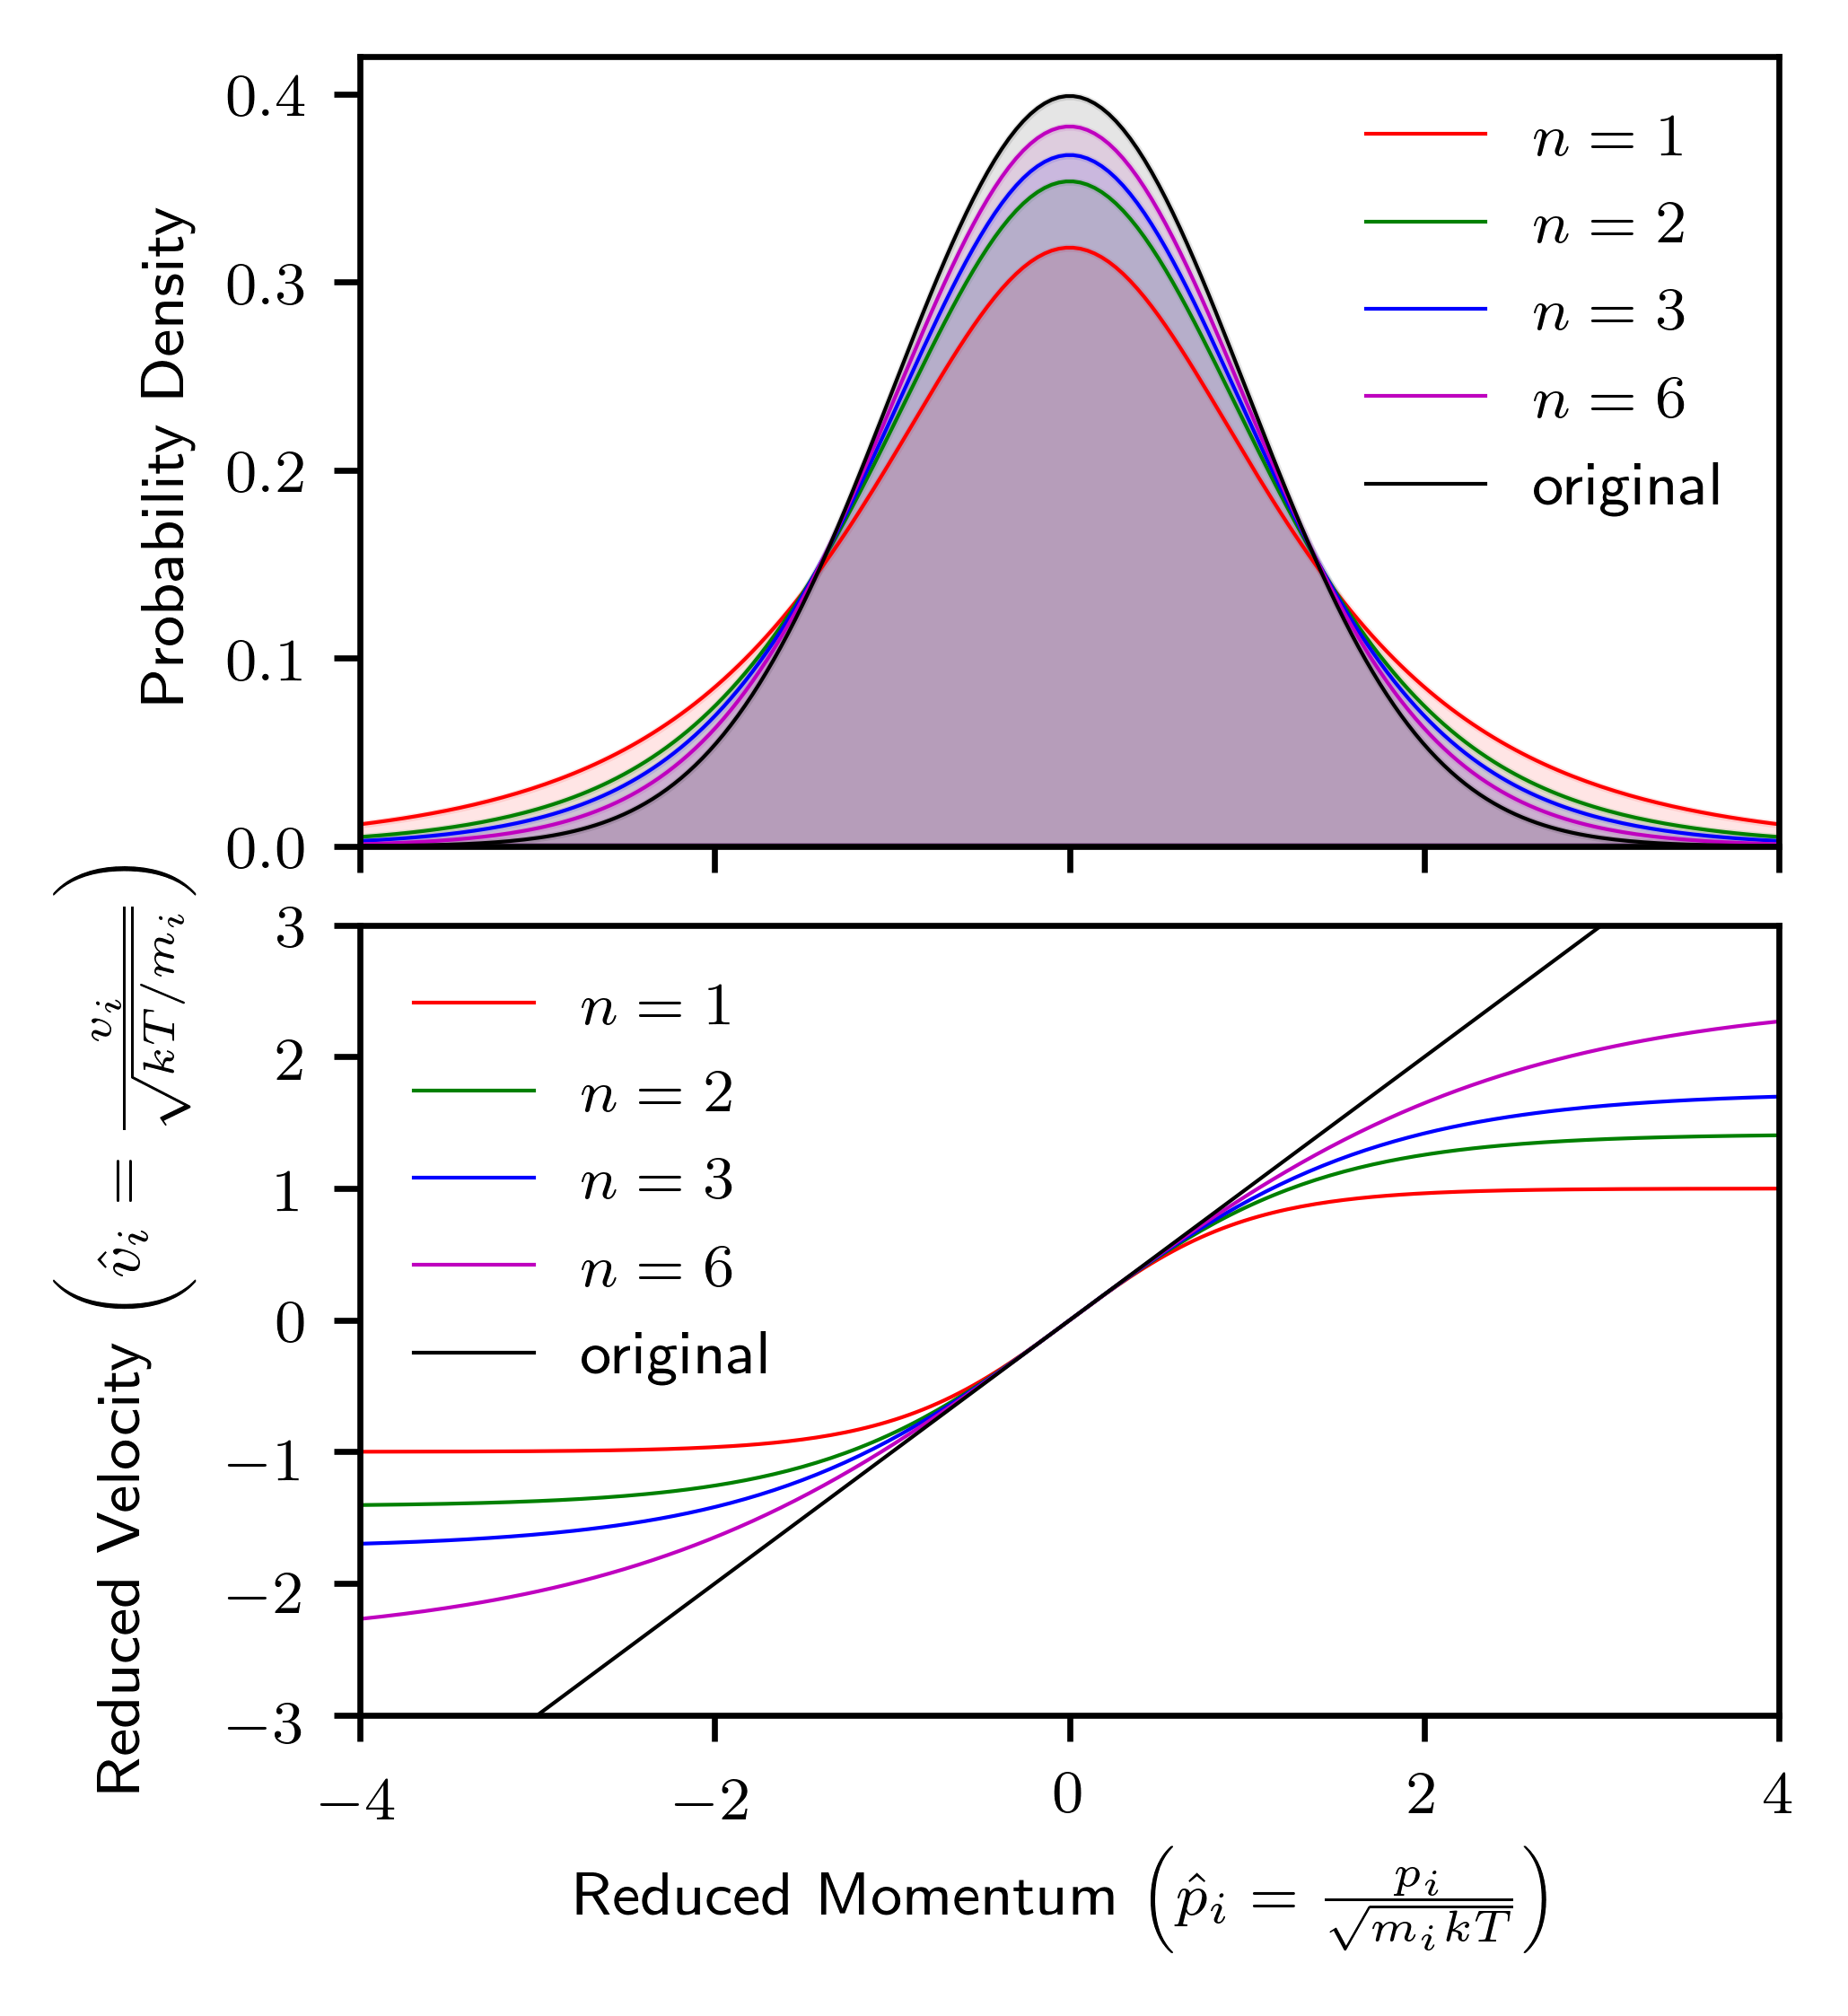
\includegraphics{momentum_functions}
	\caption{Alternative functions for expressing the momentum dependency of the Hamiltonian.}
	\label{fig:momentum distributions and velocity definition}
\end{figure}

In most NVT dynamics methods,
%such as Nos\'{e}-Hoover chains \cite{Martyna_1992} and Langevin dynamics \cite{}
the velocity of a particle is the gradient of the Hamiltonian with respect to its momentum.
With $\mathcal{H}_n$, we would have
\begin{equation}
\label{eq:velocity definition}
v_i = \diff{p_i}{{\mathcal H}_n} = \sqrt{\frac{\nn k T}{m_i}} \tanh\left(\frac{p_i}{\sqrt{\nn m_i k T}}\right).
\end{equation}

A graphics showing how velocity changes with momentum is presented in Fig.~\ref{fig:momentum distributions and velocity definition}(b).
Note that the new Hamiltonian make $v_i$ hit a plateau when $p_i$ gets too large.
This is different from the standard behavior, in which $v_i$ would keep increasing indefinitely.
In fact, such feature is what provides the modified Hamiltonian with the improved resistance to resonance when employed in multiple time-scale simulations.
In a simulation with the standard Hamiltonian, a large displacement takes place if the absolute value of some momentum increases excessively due to the action of a massive force, thus causing numerical instability.
With the new Hamiltonian, however, displacements with magnitudes above a certain value will never occur.

The modified Hamiltonian shares important properties with the original one, such as being invariant to momentum sign flips, for instance.
Also, $\mathcal{H}_n$ goes to infinity when $p_i \to \pm \infty$, which is a sufficient condition \cite{Uline_2008} for the validity of Tolman's generalized equipartition theorem,
\begin{equation}
\label{eq:generalized equipartition}
\left\langle v_i p_j \right\rangle = \delta_{ij} k T,
\end{equation}
where $\delta_{ij}$ it the Kronecker delta.

It is interesting to observe the distribution of velocities, whose PDF is derived in Appendix \ref{sec:momentum and velocity distributions} and depicted in Fig.~\ref{fig:momentum distributions and velocity definition}(b) for multiple $\nn$ values.
It is given by
\begin{equation}
\label{eq:velocity distribution}
\varrho_n(v_i) =
\begin{cases}
\frac{\Gamma\left(\frac{\nn+1}{2}\right)}{\Gamma\left(\frac{\nn}{2}\right) \sqrt{\frac{\nn \pi k T}{m_i}}} \left(1-\frac{m_i v_i^2}{\nn k T}\right)^{\frac{\nn-2}{2}} & \mathrm{if} \; v_i^2 \leq \frac{\nn k T}{m_i} \\
0 & \mathrm{otherwise}
\end{cases}.
\end{equation}

\begin{figure}
	\centering
	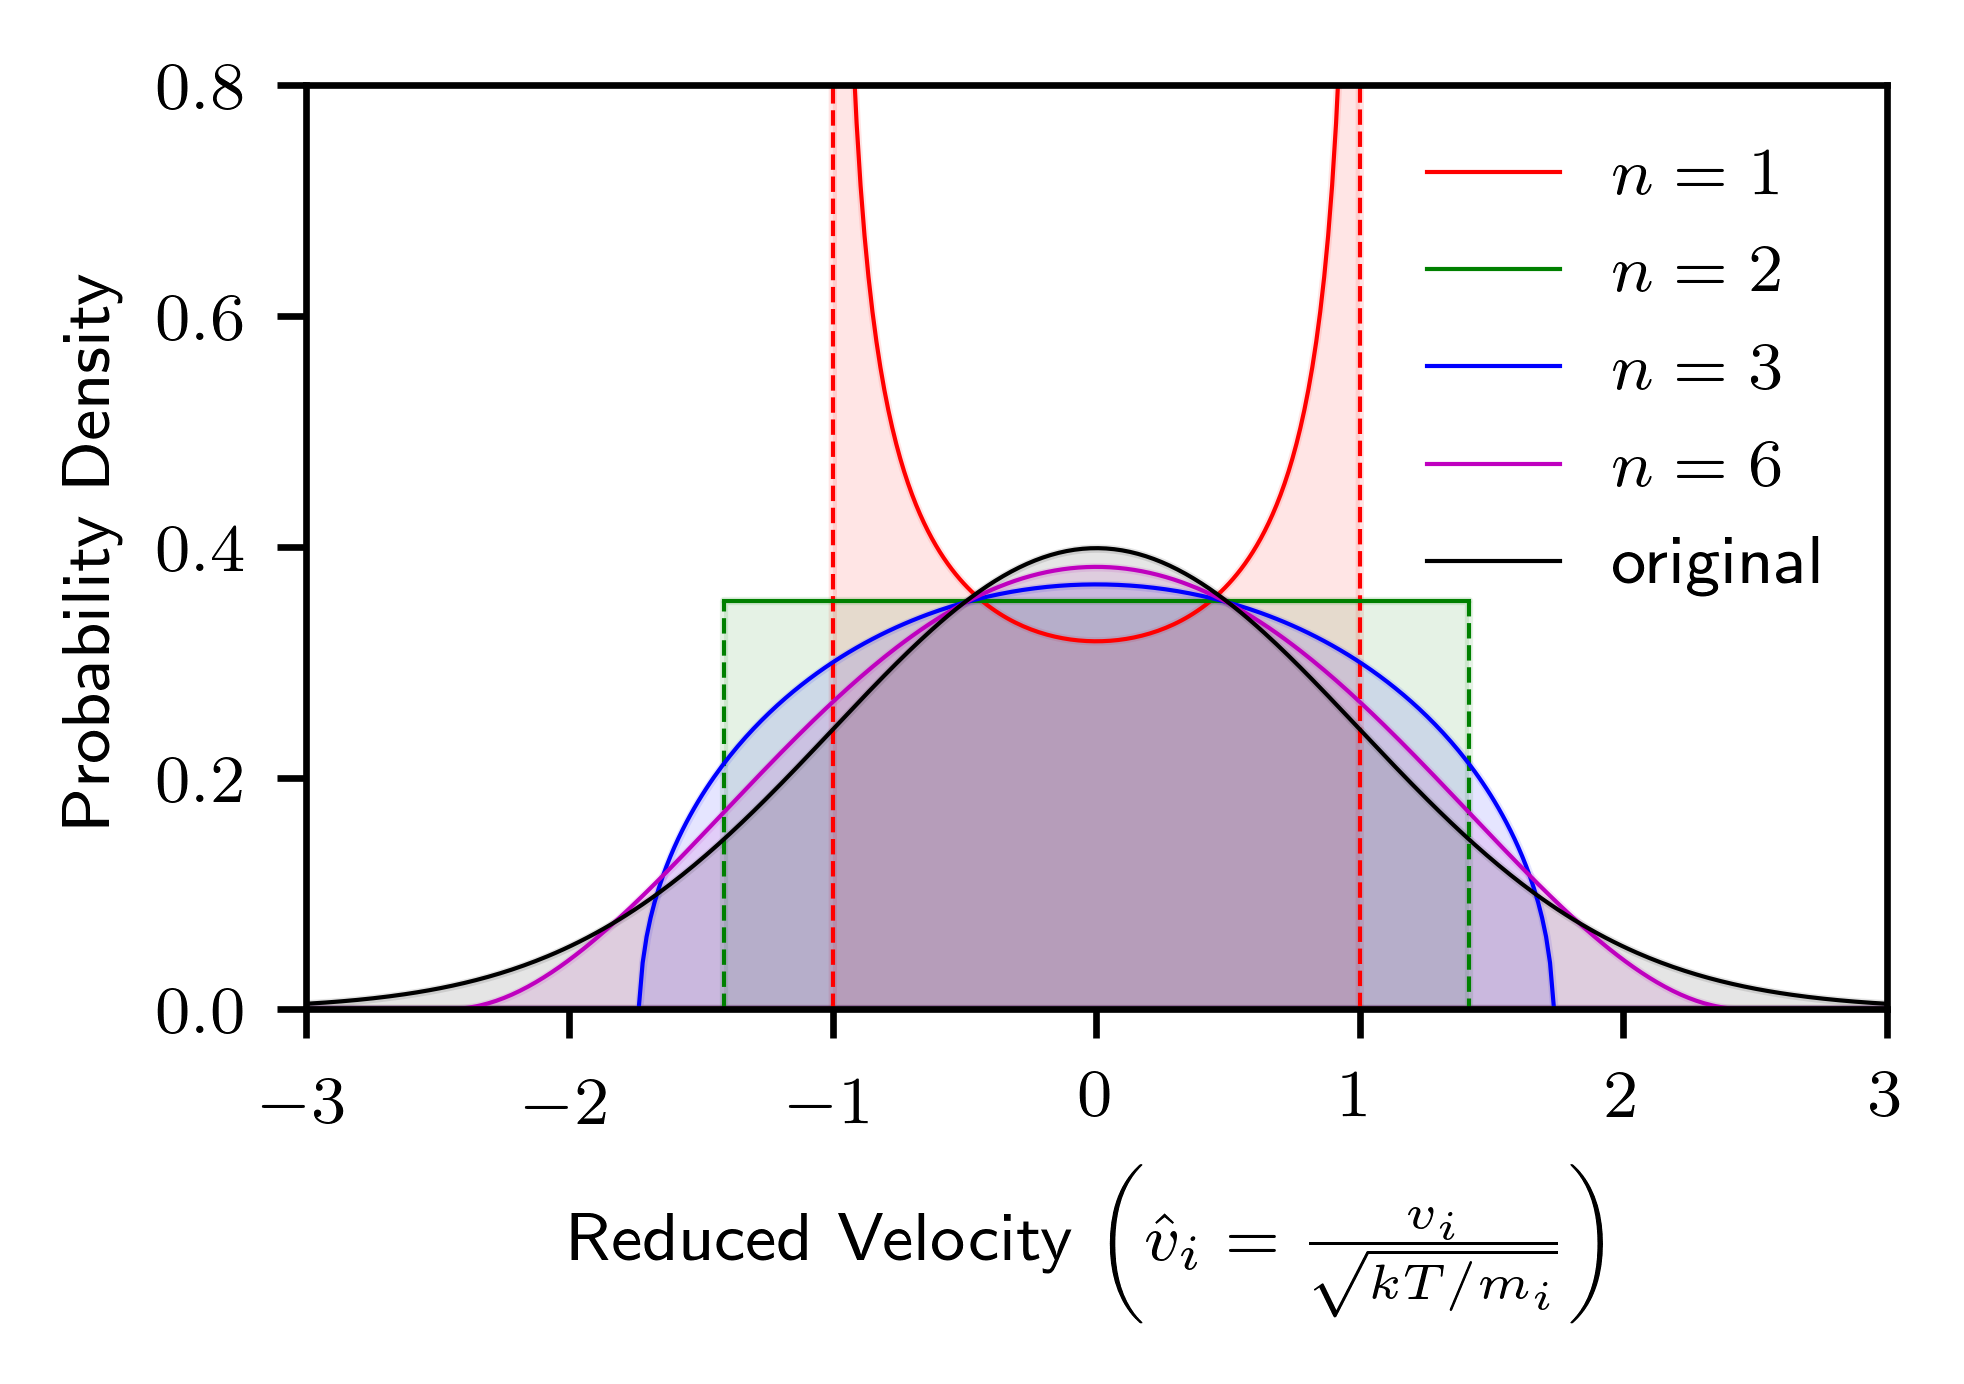
\includegraphics{velocity_distributions}
	\caption{Alternative functions for expressing the momentum dependency of the Hamiltonian.}
	\label{fig:velocity distributions}
\end{figure}

This function is akin to using Student's t-distribution with a negative degree-of-freedom parameter.
As seen in Fig.~\ref{fig:momentum distributions and velocity definition}(b), it exhibits an odd behavior for $\nn \leq 3$, but this seems to have little practical implications, as will be shown in Sec.~\ref{sec:results}.
One important aspect, which will be essential in the forthcoming discussion about thermostat algorithms, is the relation between temperature and the mean-square velocity of each degree of freedom.
From the developments in Appendix~\ref{sec:momentum and velocity distributions}, it follows that
\begin{equation}
\label{eq:mean-square velocity}
\left\langle v_i^2 \right\rangle = \frac{\nn}{\nn+1} \frac{kT}{m_i},
\end{equation}
which converges to the well-known equipartition equation when $\nn \to \infty$, as expected.

\subsection{Massive Nos\'{e}-Hoover Chain Thermostatting}
\label{sec:massive NHC thermostatting}

In a first effort to derive equations of motion for NVT dynamics with the speed-limiting Hamiltonian, we employ a massive-thermostatting version of the Nos\'{e}-Hoover chain (NHC) method \cite{Martyna_1992}.
It starts by defining an extended phase space with $m \times N_f$ extra coordinates $\vt \eta$ and their conjugate velocities $\vt v_\eta$, where $m$ is the number of thermostats in the chain attached to each degree of freedom.
It is possible to apply the method in the way it is usually presented, with the equations of motion written in terms of particle momenta.
For this, we define a quantity $H_n$ to be conserved in place of the Hamiltonian $\mathcal{H}_n$, which is
\begin{equation*}
%H_n = {\mathcal H}_n + \sum_{j=1}^m \sum_{i=1}^{N_f} \left(k T \eta_{j, i} + \frac{p_{\eta_{j, i}}^2}{2 Q} \right),
H_n = {\mathcal H}_n + \sum_{i=1}^{N_f} \sum_{j=1}^m \left(k T \eta_{j, i} + \frac{Q v_{\eta_{j, i}}^2}{2} \right),
\end{equation*}
where $Q = kT \tau^2$ is an inertial parameter derived from a characteristic time scale $\tau$.
Equations of motion devised to preserve $H_n$ can be written in the general form \cite{Sergi_2001}
\begin{equation*}
\dot{\vt x} = {\mt B} \nabla_{\vt x}{H_n},
\end{equation*}
where $\mt B$ is a skew-symmetric, matrix-valued function of the dynamic variables in $\vt x$.
%The reason is that, by virtue of the chain rule, the time derivative of a scalar function $f(\vt x)$ is given by $\dot f = \tr{\dot{\vt x}}\diff{\vt x}{f} = \tr{(\diff{\vt x}{H_n})}\tr{\mt B}\diff{\vt x}{f}$. 
%If $f = H_n$, then we have a quadratic form, which is identically null if $\tr{\mt B} = -{\mt B}$.
%The particular form of the NHC system of equations is
%\begin{subequations}
%	\label{eq:general NHC}
%	\begin{align}
%	&\dot{r}_i = \diff{p_i}{H_n} \\
%	&\dot{p}_i = -\diff{r_i}{H_n} -p_i \diff{p_{\eta_{1,i}}}{H_n} \label{eq:general NHC p} \\
%	&\dot{\eta}_{j, i} = \diff{p_{\eta_{j, i}}}{H_n} \\
%	&\dot{p}_{\eta_{1, i}} = p_i \diff{p_i}{H_n} - \diff{\eta_{1, i}}{H_n} - p_{\eta_{1, i}} \diff{p_{\eta_{2, i}}}{H_n} \label{eq:general NHC p_eta_1} \\
%	&\dot{p}_{\eta_{j, i}} = p_{\eta_{j-1, i}} \diff{p_{\eta_{j-1, i}}}{H_n} - \diff{\eta_{j, i}}{H_n} - p_{\eta_{j, i}} \diff{p_{\eta_{j+1, i}}}{H_n} \\
%	&\dot{p}_{\eta_{m, i}} = p_{\eta_{m-1, i}} \diff{p_{\eta_{m-1, i}}}{H_n} - \diff{\eta_{m, i}}{H_n}
%	\end{align}
%\end{subequations}
After all derivatives of $H_n$ have been evaluated, the particular form of the massive-NHC equations of motion is
%\begin{align*}
%&\dot{r}_i = v_i \\
%&\dot{p}_i = F_i - \frac{p_{\eta_{1,i}}}{Q} p_i \\
%&\dot{\eta}_{j,i} = \frac{p_{\eta_{j,i}}}{Q} \\
%&\dot{p}_{\eta_{1, i}} = m_i v_i p_i - kT - \frac{p_{\eta_{2,i}}}{Q} p_{\eta_{1, i}} \\
%&\dot{p}_{\eta_{j, i}} = \frac{p_{\eta_{j-1, i}}^2}{Q} - kT - \frac{p_{\eta_{j+1, i}}}{Q} p_{\eta_{j, i}} \\
%&\dot{p}_{\eta_{m, i}} = \frac{p_{\eta_{m-1, i}}}{Q} p_{\eta_{m-1, i}} - kT
%\end{align*}
\begin{subequations}
	\label{eq:NHC equations}
	\begin{align}
	&\dot{r}_i = v_i, \\
	&\dot{p}_i = F_i - v_{\eta_{1,i}} p_i, \label{eq:NHC equations p} \\
	&\dot{\eta}_{j,i} = v_{\eta_{j,i}}, \\
	&\dot{v}_{\eta_{1, i}} = \frac{v_i p_i - kT}{Q} - v_{\eta_{2, i}} v_{\eta_{1, i}}, \quad \mathrm{and}  \label{eq:NHC equations v_eta_1} \\
	&\dot{v}_{\eta_{j, i}} = \frac{Q v_{\eta_{j-1, i}}^2 - kT}{Q} - v_{\eta_{j+1, i}} v_{\eta_{j, i}} \quad \mathrm{for} \quad j > 1.
	\end{align}
\end{subequations}

In these equations, $v_i$ is the function of $p_i$ given by Eq.~\eqref{eq:velocity definition},
while $F_i = -\diff{r_i}{U}$ is the force acting on degree of freedom $i$.
%$G_{j, i} = Q v_{\eta_{j-1, i}}^2 - kT$ is the force that drives the corresponding thermostat,
By definition, $v_{\eta_{m+1, i}} = 0$.
Eq.~\eqref{eq:velocity definition} keeps $v_i$ from assuming any value beyond $\pm \sqrt{{\nn kT}/{m_i}}$.
Each $\eta_{j, i}$ is a driven variable, meaning that it is not actually necessary to integrate these variables unless we wish to validate some numerical procedure by checking the conservation of $H_n$.
From a theoretical standpoint, however, their presence is crucial for demonstrating that the original phase space is correctly sampled in proportion to $e^{-\frac{\mathcal{H}_n(\vt r, \vt p)}{kT}}$.

A non-Hamiltonian flow in the extended space preserves a measure identified by a metric determinant $\sqrt{g} = e^{-w(\vt x)}$, where $w(\vt x)$ satisfies the equation \cite{Tuckerman_1999, Tuckerman_2001}
\begin{equation}
\label{eq:extended space compressibility}
\dot{w} = \nabla_{\vt x} \cdot \dot{\vt x},
\end{equation}
where the divergence represents the extended space compressibility.
In the specific case of Eq.~\eqref{eq:NHC equations},
\begin{equation}
\dot{w} = -\sum_{i=1}^{N_f} \sum_{j=1}^m v_{\eta_{j,i}} = -\frac{d\eta_{\rm sum}}{dt},
\end{equation}
where $\eta_\mathrm{sum} = \sum_{i=1}^{N_f} \sum_{j=1}^m \eta_{j,i}$.
Therefore, $\sqrt{g} = e^{\eta_\mathrm{sum}}$.
As no combination of $\eta$'s other than $\eta_\mathrm{sum}$ is of primary importance \cite{Tuckerman_2001}, only $\eta_\mathrm{sum}$ is considered in our phase space analysis, in accordance with the guidelines of Ref.~\citenum{Tuckerman_2001}.
If $H_n$ is the only conserved quantity, then the partition function of the resulting ensemble can be expressed as
\begin{multline}
\label{eq:NHC defined partition function}
\Omega_\mathrm{NHC} = C_1 \int \delta\left(\mathcal{H}_n + kT\eta_{\rm sum} + K_\eta - H_n^0\right) \\
\times e^{\eta_{\rm sum}}  d{\vt r} d{\vt p} d{\vt v}_\eta d\eta_{\rm sum},
\end{multline}
where $H_n^0$ is a constant that depends on the system specification,
$K_\eta$ is the total kinetic energy of the thermostat network,
and $C_1$ is the proper statistical-mechanical prefactor.
Integrating over $\eta_\mathrm{sum}$ yields
\begin{equation}
\label{eq:NHC partition function}
\Omega_\mathrm{NHC} = \frac{C_1 e^{-\frac{H_n^0}{kT}}}{kT} \int e^{-\frac{K_\eta}{kT}} d{\vt v}_\eta \int e^{-\frac{\mathcal{H}_n}{kT}}  d{\vt r} d{\vt p} ,
\end{equation}
which is clearly canonical in the original phase space.

\subsection{Modified Nos\'{e}-Hoover Chain and Equivalence to the Isokinetic-NHC Method}
\label{sec:modified NHC thermostatting}

%Because
%\begin{equation}
%\delta\left(g(z)\right) = \frac{\delta(z - z_0)}{|g^\prime(x_0)|},
%\end{equation}
%where $z_0$ is a root of $g(z)$, we can rewrite Eq.~\eqref{eq:NHC defined partition function} as
%\begin{equation}
%\label{eq:NHC partition function}
%\Omega = \int d\vt x \frac{\delta\left(\eta_{\rm sum} + \frac{\mathcal{H}_n + K_\eta - C}{kT}\right)}{kT}e^{\eta_{\rm sum}},
%\end{equation}

In Eq.~\eqref{eq:NHC equations}, thermostatting is enacted by the generalized equipartition theorem, expressed in Eq.~\eqref{eq:generalized equipartition}.
Nevertheless, in order to establish the equivalence between our proposition and the isokinetic approach, some modifications in the NHC equations are necessary.
This is so because the principle that enables thermostatting in the isokinetic method is Eq.~\eqref{eq:mean-square velocity}, rather than Eq.~\eqref{eq:generalized equipartition}.
The first modification consists in substituting $m_i v_i$ for the factor $p_i$ in both Eqs.~\eqref{eq:NHC equations v_eta_1} and \eqref{eq:NHC equations p}.
Next, in order to comply with Eq.~\eqref{eq:mean-square velocity}, we multiply $m_i v_i^2$ by $\frac{\nn+1}{\nn}$ in the resulting thermostat equation.
Note that, with these changes, the dynamics still approaches the original NHC algorithm with a standard Hamiltonian when $\nn \to \infty$.
For a finite $\nn$, however, the skew-symmetric structure of matrix $\mt B$ is broken, meaning that $H_n$ will no longer be conserved.
The extended-space compressibility changes as well, but we will show that the stationary distribution correctly projects into the original phase space as proportional to $e^{-\frac{\mathcal{H}_n(\vt r, \vt p)}{kT}}$.
This requires introducing a new driven variable for every degree of freedom $i$, in substitution to the set of $\eta$ variables.
Once again, one does not need to integrate these driven variables in practice, but they are key for attesting the correctness of the method.
The new equations of motion are
\begin{subequations}
	\label{eq:isokinetic NHC equations}
	\begin{align}
	&\dot{r}_i = v_i, \\
	&\dot{p}_i = F_i - v_{\eta_{1,i}} m_i v_i, \label{eq:isokinetic NHC equations p} \\
	&\dot{\theta}_i = -\left(F_i - v_{\eta_{1,i}} m_i v_i\right)\frac{v_i \theta_i}{k T}, \label{eq:isokinetic NHC equations theta} \\
	&\dot{v}_{\eta_{1, i}} = \frac{\frac{\nn+1}{\nn} m_i v_i^2 - kT}{Q} - v_{\eta_{2, i}} v_{\eta_{1, i}}, \quad \mathrm{and} \label{eq:isokinetic NHC equations v_eta_1} \\
	&\dot{v}_{\eta_{j, i}} = \frac{Q v_{\eta_{j-1, i}}^2 - kT}{Q} - v_{\eta_{j+1, i}} v_{\eta_{j, i}} \quad \mathrm{for} \quad j > 1. \label{eq:adapted NHC equations v_eta_j}
	\end{align}
\end{subequations}

Note that $\theta_i$ can never switch sign because its own rate of change vanishes when its value approaches zero.
Here we will consider that $\theta_i$ is always positive, by convention.
The equations above have two very important properties.
First, the metric determinant they imply is given by
\begin{equation}
\label{eq:isokinetic NHC metric determinant}
\sqrt{g} = e^{-\frac{U + K_\eta}{kT}}.
\end{equation}

Second, a new conservation law emerges for every degree of freedom $i$, with a preserved quantity given by
\begin{equation}
\label{eq:isokinetic NHC conserved quantity}
\Phi_i = \theta_i \cosh^\nn\left(\frac{p_i}{\sqrt{\nn m_i k T}}\right).
\end{equation}

Mathematical proofs of both properties are provided in Appendix~\ref{sec:adapted NHC proofs}.
Even though each $\theta_i$ is a driven variable, its presence in a conservation law that involves a true dynamic variable enforces its inclusion in the phase space analysis \cite{Tuckerman_2001}.
As a consequence, the partition function of the extended-space ensemble defined by Eq.~\eqref{eq:isokinetic NHC equations} becomes
\begin{multline*}
\label{eq:isokinetic NHC defined partition function}
\Omega_\mathrm{NHC}^\ast = C_2 \int \prod_{i=1}^{N_f}\delta\left(\theta_i \cosh^\nn\left(\tfrac{p_i}{\sqrt{\nn m_i k T}}\right) - \Phi_i^0\right) \\
\times  e^{-\frac{U + K_\eta}{kT}} d{\vt r} d{\vt p} d{\vt v}_\eta d{\vt \theta}.
\end{multline*}

Integration over all $\theta$'s then makes
\begin{equation*}
\label{eq:isokinetic NHC partition function}
\Omega_\mathrm{NHC}^\ast = C_2 \int e^{-\frac{K_\eta}{kT}} d{\vt v}_\eta \int \frac{e^{-\frac{U}{kT}}}{\prod_{i=1}^{N_f} \cosh^\nn\left(\tfrac{p_i}{\sqrt{\nn m_i k T}}\right)} d{\vt r} d{\vt p}.
\end{equation*}

Due to the definition of $\mathcal{H}_n$ in Eq.~\eqref{eq:modified hamiltonian}, it is straightforward to conclude that the equation above and Eq.~\eqref{eq:NHC partition function} are equivalent.
Therefore, numerically integrating either the standard or the modified NHC equations will provide samples of the same ensemble, at least in the limit of small time steps.
Only small changes are required in well-established NHC integration methods based on operator splitting \cite{Martyna_1996, Tuckerman_2010}.
Details are given in Sec.~\ref{sec: numerical integration}.

We now demonstrate that Eq.~\eqref{eq:isokinetic NHC equations} yields the same projected dynamics in the physical phase space as the Isokinetic-NHC method of \citeauthor{Minary_2004} \cite{Minary_2004}.
We start by eliminating $p_i$ from the system by means of its relation with $v_i$.
In order to apply the chain rule $\dot{v}_i = \diff{p_i}{v_i} \dot{p}_i$, we deduce from Eq.~\eqref{eq:velocity definition} that
\begin{equation}
\label{eq:velocity derivative wrt momentum}
\frac{d v_i}{d p_i} = \frac{1}{m_i} \left(1 - \frac{m_i v_i^2}{\nn k T}\right).
\end{equation}

Then, application to Eq.~\eqref{eq:isokinetic NHC equations p} yields
\begin{equation}
\label{eq:v-based NHC equation}
\dot{v}_i = \frac{F_i}{m_i} - \frac{F_i v_i + v_{\eta_{1,i}} (\nn k T - m_i v_i^2)}{\nn k T} v_i.
\end{equation}

Next, we replace $\theta_i$ in Eq.~\eqref{eq:isokinetic NHC equations} by a new driven variable simply defined as $u_i = \sqrt[\nn]{\theta_i}$.
Because $\dot{u}_i = \frac{\dot{\theta}_i}{\nn \theta_i} u_i$,
we can substitute $\dot{\theta}$ from Eq.~\eqref{eq:isokinetic NHC equations theta} to obtain
\begin{equation}
\label{eq:u equation of motion}
\dot{u}_i = -\frac{F_i v_i - v_{\eta_{1,i}} m_i v_i^2}{\nn kT} u_i.
\end{equation}

By noting similarities in Eqs.~\eqref{eq:v-based NHC equation} and \eqref{eq:u equation of motion}, we rewrite them respectively as
\begin{subequations}
\label{eq:original isokinetic equations}
\begin{align}
&\dot{v}_i = \frac{F_i}{m_i} - \lambda_i v_i \quad \mathrm{and} \\
&\dot{u}_i = -(\lambda_i - v_{\eta_{1,i}}) u_i,
\end{align}
\end{subequations}
where $\lambda_i = \frac{F_i v_i + v_{\eta_{1,i}} (\nn k T - m_i v_i^2)}{\nn k T}$.
%\begin{equation}
%\label{eq:lambda definition}
%\lambda_i = \frac{F_i v_i + v_{\eta_{1,i}} (\nn k T - m_i v_i^2)}{\nn k T}.
%\end{equation}
%
As we can now demonstrate, these turn out to be the same equations of the method of Ref.~\citenum{Minary_2004} (with $v_{2,i} = -v_{\eta_{1,i}}$).
If an initial value is assigned to each $u_i$ so as to satisfy
\begin{equation}
\label{eq:isokinetic statement}
m_i v_i^2 + \alpha u_i^2 = \nn kT,
\end{equation}
where $\alpha$ is an arbitrary parameter, then this equality will hold forever.
This can be easily grasped if we use Eq.~\eqref{eq:original isokinetic equations} to obtain
\begin{equation*}
m_i v_i \dot{v}_i + \alpha u_i \dot{u}_i = (v_{\eta_{1,i}} - \lambda_i)(m_i v_i^2 + \alpha u_i^2 - \nn k T),
\end{equation*}
which is twice the time-derivative of $m_i v_i^2 + \alpha u_i^2$.
Hence, this derivative remains null if Eq.~\eqref{eq:isokinetic statement} holds.

Eq.~\eqref{eq:isokinetic statement} is an isokinetic statement involving $v_i$ and $u_i$.
We name it this way, instead of a constraint, because $u_i$ is not a true dynamic variable.
However, the same equation was imposed from the outset in the derivation of the original Isokinetic NHC method \cite{Minary_2004}, with $\lambda_i$ serving as a Lagrange multiplier to be determined afterwards.
Actually, instead of defining a single variable $u_i$ per degree of freedom, $\nn$ variables $u_{j, i}$ were introduced so that $\frac{\nn}{\nn+1} Q_u \sum_{j=1}^\nn u_{j, i}^2 = \alpha u_i^2$, where $Q_u$ is an inertial parameter.
In this case, the isokinetic equation becomes
\begin{equation}
m_i v_i^2 + \frac{\nn}{\nn+1} Q_u \sum_{j=1}^\nn u_{j, i}^2 = \nn kT.
\end{equation}

Finally, by using this equation to displace $m_i v_i^2$ from Eq.~\eqref{eq:isokinetic NHC equations v_eta_1}, we end up with a convenient form
\begin{equation}
\dot{v}_{\eta_{1, i}} = \frac{nkT - Q_u \sum_{j=1}^\nn u_{j, i}^2}{Q} - v_{\eta_{2, i}} v_{\eta_{1, i}}.
\end{equation}

This represents a single Nos\'{e}-Hoover chain attached to the variables $u_{j, i}$ for a fixed $i$ altogether.
In the isokinetic method \cite{Minary_2004}, however, a massive thermostatting strategy is employed at this level as well, meaning that an independent thermostat chain is attached to each $u_{j, i}$.
Even though this seems beneficial in terms of ergodicity, such a high degree of granularity might be overkill in most practical situations.
%Besides, it has the drawback of turning the $u$'s into actual dynamic (i.e. non-driven) variables.

\subsection{Massive Nos\'{e}-Hoover-Langevin Thermostat and the SIN(R) Method}
\label{sec:nose-hoover-langevin}

In the preceding section, we unveiled the connection between the Isokinetic-NHC method \cite{Minary_2004} and the use of a standard Nos\'{e}-Hoover chain algorithm in conjunction with the proposed speed-limiting Hamiltonian.
It is straightforward to extend these findings to the case in which all but the first thermostat in each chain is replaced by a single Langevin-type thermostat.
We refer to this strategy as a massive-thermostatting version of the Nos\'{e}-Hoover-Langevin (NHL) \cite{Samoletov_2007, Leimkuhler_2009} approach.
In its traditional form, it corresponds to replacing Eq.~\eqref{eq:NHC equations} by an It\={o} stochastic differential equation (SDE) system expressed as
\begin{subequations}
	\label{eq:NHL equations}
	\begin{align}
	&dr_i = v_i dt, \\
	&dp_i = F_i dt - v_{\eta_{1,i}} p_i dt, \quad \mathrm{and} \label{eq:NHL equations p} \\
	&dv_{\eta_{1, i}} = \frac{v_i p_i - kT}{Q}dt - \gamma v_{\eta_{1, i}}dt + \sigma_i dW_i,  \label{eq:NHL equations v_eta_1}
	\end{align}
\end{subequations}
where
$\sigma_i = \sqrt{2 \gamma kT / Q}$,
$\gamma$ is a friction constant,
and $dW_i$ denotes an infinitesimal increment of a Wiener process.
Note that, as in Eq.~\eqref{eq:NHC equations}, generalized equipartition is what enables proper thermostatting.
It is also possible to derive a stochastic version of the modified NHC method of Sec.~\ref{sec:modified NHC thermostatting}, in which Eq.~\eqref{eq:mean-square velocity} plays such role instead.
For this, we replace the deterministic system in Eq.~\eqref{eq:isokinetic NHC equations} by
\begin{subequations}
	\label{eq:SIN(R) equations}
	\begin{align}
	&dr_i = v_i dt, \\
	&dp_i = F_i dt - v_{\eta_{1,i}} m_i v_i dt, \quad \mathrm{and} \label{eq:SIN(R) equations p} \\
	&dv_{\eta_{1, i}} = \frac{\frac{\nn+1}{\nn} m_i v_i^2 - kT}{Q} dt - \gamma v_{\eta_{1, i}} dt + \sigma_i dW_i.
	\end{align}
\end{subequations}

The analysis of Sec.~\ref{sec:modified NHC thermostatting} also applies for SDE system above.
This is sufficient to assert its almost equivalence to the Stochastic Isokinetic Nos\'{e}-Hoover RESPA [SIN(R)] method of \citeauthor{Leimkuhler_2013} \cite{Leimkuhler_2013}, which has been proven to correctly sample the Boltzmann-Gibbs distribution of coordinates.
In fact, the method is not exactly equivalent to SIN(R) only because a single NH chain per degree of freedom is used regardless of the value of $\nn > 1$.
In addition, our analysis leads to the new conclusion that the momentum and velocity distributions that result from the SIN(R) equations are those shown in Figs.~\ref{fig:momentum distributions and velocity definition} and \ref{fig:velocity distributions} and expressed respectively by Eqs.~\eqref{eq:momentum distribution} and \eqref{eq:velocity distribution}.
In the method's name, RESPA refers to the multiple time scale integration of the equations of motion using the reversible reference system propagation algorithm \cite{Tuckerman_1992}.

\subsection{Numerical Integration}
\label{sec: numerical integration}

All methods described in the preceding sections are meant to avoid resonance in multiple time-scale (MTS) integration procedures.
%There are numerous possible ways of devising a multiple time-scale (MTS) integration procedure.
%However, we adopt here some restraints to avoid excessive intricacy.
To come up with integrators by using the reference system propagator algorithm (RESPA) \cite{Tuckerman_1992}, we can split the force on each degree of freedom $i$ into a sum of $M$ terms, i.e.
\begin{equation*}
F_i = \sum_{k=1}^M F_i^{[k]}.
\end{equation*}

By convention, the characteristic time scale of each force component increases with index $k$, meaning that $F_i^{[1]}$ is the fastest component while $F_i^{[M]}$ is the slowest one.
In the basic RESPA recipe, integration within the largest time scale ($k=M$) is done by executing $n_M$ steps of size $\delta t_M = \Delta t$.
Internally, every step of size $\delta t_k$, taken at a time scale $k$, involves $n_{k-1}$ substeps of size $\delta t_k/n_{k-1}$ each.

In general, coordinate moves are performed at the same time scale of the fastest forces.
It is possible, though, to factorize them even further, especially if they are interwoven with the handling of extended space variables.
This is done, for instance, when the coordinate moves are required to follow a geodesic motion along a constrained manifold \cite{Leimkuhler_2016}.
For simplicity, however, we will not consider this possibility in our formulation.

By writing the equations of motion in an extended space as $\dot{\vt x} = \Liu \vt x$, where $\Liu$ represents a Lie derivative (or the non-Hamiltonian extension of a Liouville operator), we can carry out a partition like
\begin{equation}
\label{eq:RESPA Liouville Partition}
\Liu = \Liu_\mathrm{A} + \underbrace{\sum_{k=1}^M \Liu_\mathrm{B}^{[k]}}_{\Liu_\mathrm{B}} + \underbrace{\sum_{k=0}^M \Liu_\mathrm{bath}^{[k]}}_{\Liu_\mathrm{bath}},
\end{equation}
where $\Liu_\mathrm{A}$ is the only component which entails changes in the particle coordinates,
$\Liu_\mathrm{B}^{[k]}$ is the only one that depends on the forces labeled with superscript $k$, and
$\Liu_\mathrm{bath}^{[k]}$ entails transformations in particle momenta that depend exclusively on the state of thermostat-related variables.
Transformations in these variables themselves can occur due to the action of any component in Eq.~\eqref{eq:RESPA Liouville Partition}.
The propagator representing a relatively general RESPA scheme can be written as a recursive approximation based on the Trotter-Suzuki theorem \cite{Trotter_1959, Suzuki_1976}.
For this, we make
\begin{subequations}
\label{eq:RESPA propagator}
\begin{equation}
\label{eq:RESPA outermost propagator}
e^{t \Liu} \approx \mathcal{G}_M(t),
\end{equation}
where $\mathcal{G}_M$ belongs to a family of operators whose each member $\mathcal{G}_k(\delta t)$, for $k \in [1, M]$, is defined as
\begin{multline}
\label{eq:RESPA scheme 1}
\mathcal{G}_k(\delta t) = \Big[
e^{\frac{\delta t}{2 n_k} \Liu_\mathrm{bath}^{[k]}}
e^{\frac{\delta t}{2 n_k} \Liu_\mathrm{B}^{[k]}}
\mathcal{G}_{k-1}\left(\tfrac{\delta t}{n_k}\right)
\times \\ \times
e^{\frac{\delta t}{2 n_k} \Liu_\mathrm{B}^{[k]}}
e^{\frac{\delta t}{2 n_k} \Liu_\mathrm{bath}^{[k]}}
\Big]^{n_k}.
\end{multline}

Finally, the recursive process comes to an end once we make
\begin{equation}
\label{eq:RESPA innermost propagator}
\mathcal{G}_0(\delta t) = e^{\frac{\delta t}{2} \Liu_\mathrm{A}}
e^{\delta t \Liu_\mathrm{bath}^0}
e^{\frac{\delta t}{2} \Liu_\mathrm{A}}.
\end{equation}
\end{subequations}

In this general formulation, one is free to allocate the components of $\Liu_\mathrm{bath}$ throughout the several time scales, provided that $\sum_{k=0}^M \Liu_\mathrm{bath}^{[k]} = \Liu_\mathrm{bath}$.
For simplicity, however, we only consider cases in which the whole integration is done in a single time scale with selected index $k^\ast$, thus making $\Liu_\mathrm{bath}^{[k]} = 0$ for all $k \neq k^\ast$.
When $k^\ast \geq 1$, we can conveniently rewrite Eq.~\eqref{eq:RESPA innermost propagator} as $\mathcal{G}_0(\delta t) = e^{\delta t \Liu_\mathrm{A}}$.
This formulation reproduces the XO-RESPA (extended system outside-RESPA) method introduced by \citeauthor{Martyna_1996} \cite{Martyna_1996} if we make $k^\ast = M$.
Although it does not fit exactly the XI-RESPA (extended system inside-RESPA) scheme \cite{Martyna_1996}, a close variant XI\textsuperscript{*}-RESPA can be devised by making $k^\ast = 1$.

Both XO-RESPA and XI-RESPA can be considered as MTS generalizations of a scheme in which a Velocity Verlet step is surrounded by half-step integrations of the thermostat variables.
\citeauthor{Zhang_2017} \cite{Zhang_2017} have compared the performance of this single time scale method, which they referred to as the ``side'' scheme, with those of other alternatives.
One of these, called the ``middle'' scheme, can be generalized to the MTS case if we simply make $k^\ast = 0$.
This is an important advantage of the general formula of Eq.~\eqref{eq:RESPA propagator}.
Note that, in this case, the thermostat-variable integration is surrounded by coordinate moves.
In this way, thermostat-induced changes in the particle momenta acquire a more direct influence on the resulting new coordinates at every step.
As \citeauthor{Zhang_2017} observed, this tends to produce better coordinate sampling when compared to the more traditional side scheme \cite{Zhang_2017}.
This means that ensemble averages of coordinate-related properties become less affected by an increase in the time step size.
Such a tendency had been previously noticed for Langevin thermostats with the related BAOAB method \cite{Leimkuhler_2012, Leimkuhler_2013_2}, but the new study extended the observation to other stochastic as well as deterministic algorithms.
\citeauthor{Zhang_2017} \cite{Zhang_2017} also noted that, like BAOAB, the middle scheme degrades the sampling of momenta with respect to reproducing the theoretical probability distribution at the specified temperature.
In the middle-RESPA case, the numerical propagator simplifies to
\begin{subequations}
\begin{equation*}
\label{eq:middle RESPA scheme 1}
\mathcal{G}_k^\mathrm{middle}(\delta t) = \Big[
e^{\frac{\delta t}{2 n_k} \Liu_\mathrm{B}^{[k]}}
\mathcal{G}_{k-1}\left(\tfrac{\delta t}{n_k}\right)
e^{\frac{\delta t}{2 n_k} \Liu_\mathrm{B}^{[k]}}
\Big]^{n_k}
\end{equation*}
for $k \in [1, M]$ and %$\mathcal{G}_0^\mathrm{mid}(\delta t) = e^{\frac{\delta t}{2} \Liu_\mathrm{A}} e^{\delta t \Liu_\mathrm{bath}} e^{\frac{\delta t}{2} \Liu_\mathrm{A}}$.
\begin{equation*}
\label{eq:middle RESPA innermost propagator}
\mathcal{G}_0^\mathrm{middle}(\delta t) = e^{\frac{\delta t}{2} \Liu_\mathrm{A}}
e^{\delta t \Liu_\mathrm{bath}}
e^{\frac{\delta t}{2} \Liu_\mathrm{A}}.
\end{equation*}
\end{subequations}

In all cases considered here, we have
\begin{equation*}
\mathcal{L}_\mathrm{A} = \sum_{i=1}^{N_f} v_i \diff{r_i}{} \quad \mathrm{and} \quad
\mathcal{L}_\mathrm{B}^{[k]} = \sum_{i=1}^{N_f} F^{[k]}_i \diff{p_i}{}.
\end{equation*}

Thus, the effects of propagators $e^{t \mathcal{L}_\mathrm{A}}$ and $e^{t \mathcal{L}_\mathrm{B}^{[k]}}$ can be respectively expressed as $r_i = r_{i, 0} + v_{i, 0} t$ and $p_i = p_{i, 0} + F_i(\vt r_0) t$ for all $i$, where subscript $0$ stands for initial condition.
The effect of propagator $e^{t \Liu_\mathrm{bath}}$ will differ from case to case.
Let us focus on the two Nos\'{e}-Hoover-Langevin strategies described in Sec.~\ref{sec:nose-hoover-langevin}.
First, considering the equations of motion in Eq.\eqref{eq:NHL equations}, we carry out a Trotter-Suzuki splitting $e^{\delta t \Liu_\mathrm{bath}} = e^{\frac{\delta t}{2} \mathcal{L}_\mathrm{S}} e^{\delta t \mathcal{L}_\mathrm{O}} e^{\frac{\delta t}{2} \mathcal{L}_\mathrm{S}}$, where $\mathcal{L}_\mathrm{S} = - \sum_{i=1}^{N_f} v_{\eta_{1,i}} p_i \diff{p_i}{}$ alone produces the deterministic system
\begin{align*}
&\dot{r}_i = 0, \\
&\dot{p}_i = - v_{\eta_{1,i}} m_i v_i, \quad \mathrm{and} \\
&\dot{v}_{\eta_{1,i}} = 0,
\end{align*}
while $\mathcal{L}_\mathrm{O}$ generates a forced Ornestein-Uhlenbeck process defined by the stochastic system
\begin{align*}
&dr_i = 0, \\
&dp_i = 0, \quad \mathrm{and} \\
&dv_{\eta_{1, i}} = \frac{v_i p_i - kT}{Q}dt - \gamma v_{\eta_{1, i}}dt + \sigma_i dW_i.
\end{align*}

For the first equation system, the solution (and corresponding exact effect of propagator $e^{t \mathcal{L}_\mathrm{S}}$) is a momentum scaling given by
\begin{equation*}
p_i = p_{i,0} e^{-v_{\eta_{1,i,0}} t}.
\end{equation*}

From the second system, in turn, the effect of propagator $e^{t \mathcal{L}_\mathrm{O}}$ is obtained as
\begin{equation*}
v_{\eta_{1, i}} = g_i (1 - e^{-\gamma t})
+ v_{\eta_{1,i,0}} e^{-\gamma t} + \sqrt{\tfrac{kT}{Q}(1 - e^{-2\gamma t})} \xi_i,
\end{equation*}
where $\xi_i$ is an independent random variate distributed according to a standard normal probability density and $g_i = \frac{1}{Q}(v_{i,0} p_{i,0} - kT)$ is a constant force.

All these propagators are straightforward to implement once a computer code is available for computing the force components at every time scale.
In practice, it is often necessary to bound the values of $p_i$ in order to avoid numerical overflow, especially in the case of a very large external time step $\Delta t$.
Here we prepare our codes to make $p_i = \pm 15 \sqrt{n m_i kT}$ whenever the magnitude of $p_i$ exceeds this value, which can happen sporadically due to spuriously large interactions.
As one can infer from Fig.~\ref{fig:momentum distributions and velocity definition}, it is extremely unlikely that such a large departure from the mean occurs genuinely.

%\begin{gather*}
%\mathcal{L}_\mathrm{A} = \sum_{i=1}^{N_f} v_i \diff{r_i}{} \\
%\mathcal{L}_\mathrm{B}^{[k]} = \sum_{i=1}^{N_f} F^{[k]}_i \diff{p_i}{} \\
%\mathcal{L}_\mathrm{S} = - \sum_{i=1}^{N_f} v_{\eta_{1,i}} p_i \diff{p_i}{} \\
%\mathcal{L}_\mathrm{S}^\ast = - \sum_{i=1}^{N_f} v_{\eta_{1,i}} m_i v_i \diff{p_i}{} \\
%\mathcal{L}_\mathrm{DOU} = \sum_{i=1}^{N_f} \frac{v_i p_i - kT}{Q} \diff{v_{\eta_{1, i}}}{} + \mathcal{L}_\mathrm{OU} \\
%\mathcal{L}_\mathrm{DOU}^\ast = \sum_{i=1}^{N_f} \frac{\frac{\nn+1}{\nn} m_i v_i^2 - kT}{Q} \diff{v_{\eta_{1, i}}}{} + \mathcal{L}_\mathrm{OU}
%\end{gather*}

We now turn the attention to the simplified version of the SIN(R) method expressed in Eq.~\eqref{eq:SIN(R) equations}.
In this case we make $e^{\delta t \Liu_\mathrm{bath}} = e^{\frac{\delta t}{2} \mathcal{L}_\mathrm{S}^\ast} e^{\delta t \mathcal{L}_\mathrm{O}^\ast} e^{\frac{\delta t}{2} \mathcal{L}_\mathrm{S}^\ast}$, very similarly to the integration method described above.
The only difference between the effect of propagator $e^{t \mathcal{L}_\mathrm{O}^\ast}$ and that of its counterpart is in the calculation of the force, which is now given by $g_i^\ast = \frac{1}{Q}(\frac{\nn+1}{\nn} m_i v_{i,0}^2 - kT)$.
In the case of propagator $e^{t \mathcal{L}_\mathrm{S}^\ast}$, its effect can be obtained by solving
\begin{equation*}
\frac{d \hat{p}_i}{d t} = - v_{\eta_{1,i}} \sqrt{\nn} \tanh\left(\frac{\hat{p}_i}{\sqrt{\nn}}\right),
\end{equation*}
where $\hat{p}_i = \frac{p_i}{\sqrt{m_i kT}}$ is a reduced momentum and $v_{\eta_{1,i}}$ is considered to be constant.
Since $\cosh x dx = d \sinh x$ and $\cosh x \tanh x = \sinh x$, the solution turns out to be a scaling of $\sinh\left({\hat{p}_i}/{\sqrt{\nn}}\right)$.
Therefore,
\begin{equation}
\label{eq:hyperbolic sine scaling}
\hat{p}_i = \sqrt{\nn} \arcsinh\left[\sinh \left(\frac{\hat{p}_{i,0}}{\sqrt{\nn}}\right) e^{-v_{\eta_{1,i}} t}\right].
\end{equation}

It is also possible to express the solution above in terms of velocities.
After simplification by means of hyperbolic function identities, the final expression is
\begin{equation}
\label{eq:velocity scaling and renormalization}
v_i = \frac{v_{i,0} e^{-v_{\eta_{1,i}} t}}{\sqrt{\frac{\nn kT}{m_i} - v_{i,0}^2 + \left(v_{i,0} e^{- v_{\eta_{1,i}} t}\right)^2}}.
\end{equation}

This can be interpreted as a velocity scaling followed by renormalization, thus guaranteeing that the final result will lie in the allowable range.
We note that using Eq.~\eqref{eq:velocity scaling and renormalization}, together with the required transformations from $p_i$ to $v_i$ and back, is numerically more stable than using Eq.~\eqref{eq:hyperbolic sine scaling}.
%Because Eq.~\eqref{eq:isokinetic NHC equations p} is the only one in the corresponding system which directly involves the momentum $p_i$, using the equation above in the numerical integration eliminates the need to compute and store $\vt p$ altogether.

Integration of the deterministic equations of motion of Secs.~\ref{sec:massive NHC thermostatting} and \ref{sec:modified NHC thermostatting} follow similar procedures in which $e^{t \Liu_\mathrm{bath}}$ corresponds to the NHC integration method described, for instance, in Ref.~\citenum{Martyna_1996}.

\subsection{A New Method: Limited-Speed Langevin Dynamics}

The step required to evolve from the Isokinetic NHC method \cite{Minary_2004} to the SIN(R) method \cite{Leimkuhler_2013} is the same one involved in going from the original NHC algorithm \cite{Martyna_1992, Martyna_1996} to the NHL approach \cite{Samoletov_2007, Leimkuhler_2009}.
It consists in attaching a stochastic thermostat, instead of a chain of deterministic ones, to the Nos\'{e}-Hoover device that controls the temperature of the physical system.
Taking one step further, we can eliminate the mediation altogether and attach a stochastic thermostat directly to each physical degree of freedom.
In the case of a traditional Hamiltonian, this leads to the well-known Langevin dynamics.
Here we test how using this approach, but with a speed-limiting Hamiltonian instead, compares to the previous methods in its ability to cope with resonance artifacts.

By following \citeauthor{Stoltz_2018} \cite{Stoltz_2018}, who considered the general case in which the kinetic energy part of a separable Hamiltonian is replaced by another function of momenta, we write down a SDE system for each degree of freedom $i$ as
\begin{subequations}
	\label{eq:Langevin equations}
	\begin{align}
	&dr_i = v_i dt \quad \mathrm{and} \\
	&dp_i = F_i dt - \gamma m_i v_i dt + \sigma_i dW_i,
	\end{align}
\end{subequations}
with $\sigma_i = \sqrt{2 \gamma m_i kT}$ and $v_i$ is a function of $p_i$ such as defined in Eq.~\eqref{eq:velocity definition}.
The Gibbs-Boltzmann probability density function $\rho(\vt r, \vt p) = {Z}^{-1} e^{-\frac{\mathcal{H}_n(\vt r, \vt p)}{kT}}$ is a stationary distribution of the SDE system above because it satisfies the Fokker-Planck equation \cite{Leimkuhler_2015}
\begin{equation}
\diff{t}{\rho} = -i\!L \rho + \sum_{i=1}^{N_f} \left[ \gamma m_i \diff{p_i}{}(\rho v_i) + \frac{\sigma_i^2}{2} \diff{p_i^2}{^2 \rho} \right],
\end{equation}
where $i\!L$ is the Liouville operator corresponding to the modified Hamiltonian, for which $i\!L \mathcal{H}_n = 0$ \cite{Tuckerman_2010}.
This is so because $\diff{t}{\rho} = 0$, since there is no explicit dependence on time, and $i\!L \rho = -\frac{\rho}{kT}i\!L \mathcal{H}_n = 0$.
In addition, after evaluating the remaining derivatives, we end up with
\begin{equation}
\rho \sum_{i=1}^{N_f} \left[ \left(-\gamma m_i + \frac{\sigma_i^2}{2 kT}\right) \left(\frac{v_i^2}{kT} - \frac{d v_i}{d p_i}\right) \right] = 0,
\end{equation}
which is identically satisfied since $\sigma_i^2 = 2 \gamma m_i kT$.

There are several numerical methods available in the literature for solving the standard Langevin equation, in which $v_i(p_i) = p_i/m_i$.
However, adjustment is required for them to become usable for solving Eq.~\eqref{eq:Langevin equations}.
We select the BAOAB integrator \cite{Leimkuhler_2012, Leimkuhler_2013_2} as our starting point due to its outstanding efficiency in reproducing canonical statistics of configurations, termed as a superconvergence property \cite{Leimkuhler_2012}.
In the single time-scale case, it consists in applying, at each time step of size $\delta t$, a split propagator defined as
\begin{equation}
e^{\delta t \mathcal{L}_\textsc{BAOAB}} =
e^{\frac{\delta t}{2} \mathcal{L}_\mathrm{B}}
e^{\frac{\delta t}{2} \mathcal{L}_\mathrm{A}}
e^{\delta t \mathcal{L}_\mathrm{O}}
e^{\frac{\delta t}{2} \mathcal{L}_\mathrm{A}}
e^{\frac{\delta t}{2} \mathcal{L}_\mathrm{B}},
\end{equation}
whose each factor represents the exact solution of a simpler subproblem.
The division can be depicted \cite{Leimkuhler_2015} as
\begin{equation}
\left[\begin{array}{c}
dr_i \\ dp_i
\end{array}\right] =
\underbrace{\left[\begin{array}{c}
v_i dt \\ 0
\end{array}\right]}_\mathrm{A} + 
\underbrace{\left[\begin{array}{c}
0 \\ F_i dt
\end{array}\right]}_\mathrm{B} +
\underbrace{\left[\begin{array}{c}
0 \\ -\gamma m_i v_i dt + \sigma_i dW_i
\end{array}\right]}_\mathrm{O}.
\end{equation}

The effects of propagators $e^{\delta t \mathcal{L}_\mathrm{A}}$ and $e^{\delta t \mathcal{L}_\mathrm{B}}$ were explained in Sec.~\ref{sec: numerical integration}.
In the traditional case, the remaining propagator, $e^{t \mathcal{L}_\mathrm{O}}$, represents an Ornstein-Uhlenbeck (OU) process and, as such, its effect can be evaluated exactly (in the stochastic sense) from a closed-form solution of the linear SDE
\begin{equation}
\label{eq:traditional Langevin}
d\hat{p}_i = - \gamma \hat{p}_i dt + \sqrt{2 \gamma} dW_i,
\end{equation}
which is
\begin{equation}
\label{eq:Ornestein-Uhlenbeck solution}
\hat{p}_i = e^{-\gamma t} \hat{p}_{i,0} + \sqrt{1 - e^{-2 \gamma t}} \xi_i.
\end{equation}

In the present case, however, this propagator represents the joint solution, for all $i$, of a non-linear stochastic process given by
\begin{equation}
\label{eq:Langevin equation with new velocity}
d\hat{p}_i = - \gamma \sqrt{\nn} \tanh\left(\frac{\hat{p}_i}{\sqrt{\nn}}\right) dt + \sqrt{2 \gamma} dW_i.
\end{equation}

This is not an OU process and has no simple analytical solution.
Some approximation is thus required.
In the present work, we consider and empirically test two approximate solutions, described as follows.

\subsubsection{Non-Linear Extension of the Gr{\o}nbech-Jensen \& Farago Integrator}

The Langevin integrator proposed by \citeauthor{Gronbech-jensen_2013} \cite{Gronbech-jensen_2013} (GJF) has also been observed to show excellent performance at sampling configurations in accordance with the canonical distribution \cite{Jensen_2019, Farago_2019, Finkelstein_2019}.
A little-known fact about this integrator is its incidentally close correspondence with the BAOAB splitting (\citeauthor{Li_2017} \cite{Li_2017}, Appendix B).
In fact, it is possible to derive the GJF method by simply replacing the exact OU solution in the BAOAB scheme by a numerical approximation.
Integrating both sides of Eq.~\eqref{eq:traditional Langevin} yields
\begin{equation*}
\hat{p}_i - \hat{p}_{i,0} = - \gamma \int_0^t \hat{p}_i(s) ds + \sqrt{2 \gamma t} \xi_i.
\end{equation*}

Then, by using the trapezoidal rule to evaluate the remaining integral, we obtain
\begin{equation}
\label{eq:GJF approximation}
\hat{p}_i \approx \frac{\left(1 - \tfrac{\gamma t}{2}\right) \hat{p}_{i,0} + \sqrt{2 \gamma t} \xi_i}{1 + \tfrac{\gamma t}{2}}.
\end{equation}

Following Ref.~\citenum{Li_2017}, another possible interpretation is that GJF corresponds to using BAOAB with an approximate friction constant given by
\begin{equation*}
\gamma^\ast = -\frac{1}{\delta t} \ln \frac{1 - \tfrac{\gamma \delta t}{2}}{1 + \tfrac{\gamma \delta t}{2}}.
\end{equation*}

This explains why GJF is as accurate as BAOAB at reproducing the equilibrium statistics of harmonic oscillators \cite{Jensen_2019, Farago_2019, Finkelstein_2019}, as the latter is known to yield a coordinate-momentum covariance matrix that does not depend on the friction constant \cite{Leimkuhler_2013_2}.
It is interesting, though, that in a recent observation of molecular diffusion in the large-friction regime ($\gamma \approx  0.1~\mathrm{fs}^{-1}$), BAOAB seems to deviate from the expected diffusive behavior as the time-step size increases, whereas GJF keeps giving the correct results.
Because splitting is itself an approximation, employing a linearized step instead of its exact counterpart might be causing some error compensation.

In view of the good performance of the GJF method, the trapezoidal rule can also provide us with a solution for Eq.~\eqref{eq:Langevin equation with new velocity}.
In this case, however, the value of $\hat{p}_i$ must be computed self-consistently.
For instance, we can use
\begin{equation}
%\hat{p}_i = \hat{p}_i - \frac{\hat{p}_i + \frac{\gamma \delta t}{2} \sqrt{\nn} \tanh \left(\frac{\hat{p}_i}{\sqrt{\nn}}\right) - C}{1 + \frac{\gamma \delta t}{2} \left[1 - \tanh^2 \left(\frac{\hat{p}_i}{\sqrt{\nn}}\right) \right]},
\hat{p}_i = \hat{p}_i - \frac{\hat{p}_i + \frac{\gamma t}{2} \hat{v}_i - C_{i,0}}{1 + \frac{\gamma t}{2} \left(1 - \frac{\hat{v}_i^2}{\nn} \right)},
\end{equation}
where $\hat{v}_i = \sqrt{\nn} \tanh\left(\frac{\hat{p}_i}{\sqrt{\nn}}\right)$ and $C_{i,0} = \hat{p}_{i,0} - \frac{\gamma t}{2} \hat{v}_{i,0} + \sqrt{2 \gamma t} \xi_i$.
This comes from applying the Newton-Raphson method to a monotonic function of $\hat{p}_i$, which makes it quadratically convergent.
By employing the same value of $\xi_i$ as in the $C_{i,0}$ constant, either Eq.~\eqref{eq:Ornestein-Uhlenbeck solution} or Eq.~\eqref{eq:GJF approximation} is expected to provide a suitable initial guess.

\subsubsection{Perturbed Ornstein-Uhlenbeck Process}

By defining a perturbation function $\hat{z}_i(\hat{p}_i)$ as
\begin{equation}
z_i = \sqrt{\nn} \tanh\left(\frac{\hat{p}_i}{\sqrt{\nn}}\right) - \hat{p}_i,
\end{equation}
we can rewrite Eq.~\eqref{eq:Langevin equation with new velocity} as
\begin{equation}
\label{eq:Langevin equation with perturbed OU process}
d\hat{p}_i = \underbrace{- \gamma \hat{p}_i dt + \sqrt{2 \gamma} dW_i}_\mathrm{O} - \gamma \hat{z}_i dt.
\end{equation}

It is clear that $z_i$ is mostly relevant for small values of $\nn$, but vanishes as $\nn \to \infty$.
We propose a splitting solution for the equation above in which an exact OU step is surrounded by correction steps, that is,
\begin{equation*}
e^{t \Liu_\mathrm{bath}} =
e^{-\frac{t}{2} \mathcal{L}_\mathrm{S}}
e^{\frac{t}{2} \mathcal{L}_\mathrm{S}^\ast}
e^{t \mathcal{L}_\mathrm{O}}
e^{\frac{t}{2} \mathcal{L}_\mathrm{S}^\ast}
e^{-\frac{t}{2} \mathcal{L}_\mathrm{S}}.
\end{equation*}
%\begin{equation*}
%e^{\delta t \mathcal{L}_\mathrm{O}} =
%e^{\frac{\delta t}{2} \gamma \hat{\vt p} \cdot \nabla_{\hat{\vt p}}}
%e^{-\frac{\delta t}{2} \gamma \hat{\vt v} \cdot \nabla_{\hat{\vt p}}}
%e^{\delta t \mathcal{L}_\mathrm{OU}}
%e^{-\frac{\delta t}{2} \gamma \hat{\vt v} \cdot \nabla_{\hat{\vt p}}}
%e^{\frac{\delta t}{2} \gamma \hat{\vt p} \cdot \nabla_{\hat{\vt p}}}.
%\end{equation*}

\citeauthor{Stoltz_2018} \cite{Stoltz_2018} have shown that splitting solutions applied to stochastic equations such as Eq.~\eqref{eq:Langevin equation with new velocity} can converge to a stationary distribution because $|\hat{v}_i - \hat{p}_i|$ 

\cite{Trstanova_2016}

considered the convergence of


we can expect that will converge to a stationary distribution, since $| m_i v_i - p_i |$ is bounded.


\begin{equation}
e^{\frac{\delta t}{2} \mathcal{L}_{Z}} =
e^{\frac{\delta t}{4} \gamma \hat{p}_i \diff{\hat{p}_i}{}}
e^{-\frac{\delta t}{2}  \gamma \hat{v}_i \diff{\hat{p}_i}{}}
e^{\frac{\delta t}{4} \gamma \hat{p}_i \diff{\hat{p}_i}{}}
\end{equation}

\begin{equation*}
e^{\delta t \mathcal{L}_\mathrm{O}} =
e^{\frac{\delta t}{2} \gamma \hat{\vt p} \cdot \nabla_{\hat{\vt p}}}
e^{\frac{\delta t}{2} \gamma \hat{\vt v} \cdot \nabla_{\hat{\vt p}}}
e^{\delta t \mathcal{L}_\mathrm{OU}}
e^{\frac{\delta t}{2} \gamma \hat{\vt v} \cdot \nabla_{\hat{\vt p}}}
e^{\frac{\delta t}{2} \gamma \hat{\vt p} \cdot \nabla_{\hat{\vt p}}}
\end{equation*}


By composing the three steps in a single equation, the effect of propagator $e^{\delta t \mathcal{L}_{Z}}$ can be represented by
\begin{equation*}
\hat{p}_i(t+\delta t) = e^{\frac{\gamma \delta t}{2}} \sqrt{\nn} \arcsinh\left[\sinh\left(\frac{\hat{p}_i(t) e^{\frac{\gamma \delta t}{2}}}{\sqrt{\nn}}\right) e^{-\gamma \delta t} \right].
\end{equation*}

Unfortunately, linear analysis is not possible.

\section{Results}
\label{sec:results}

\subsection{Numerical Integration of the Modified Stochastic Propagator}

In order to have a proper 

Order-1.5 Strong It\={o}-Taylor Scheme \cite{Kloeden_1992}
\begin{multline}
p_i = \hat{p}_{i,0} - \hat{v}_{i,0} \gamma t + \sqrt{2 \gamma t} \xi_{i,1} - \left(1 - \frac{\hat{v}_{i,0}^2}{\nn}\right) \times \\
\times \left[ \frac{\sqrt{2 \gamma^3 t^3}}{2}\left(\xi_{i,1} + \frac{\xi_{i,2}}{\sqrt{3}}\right) - \frac{\nn+2}{2 \nn} \hat{v}_{i,0} \gamma^2 t^2 \right],
\end{multline}

\begin{figure}
	\centering
	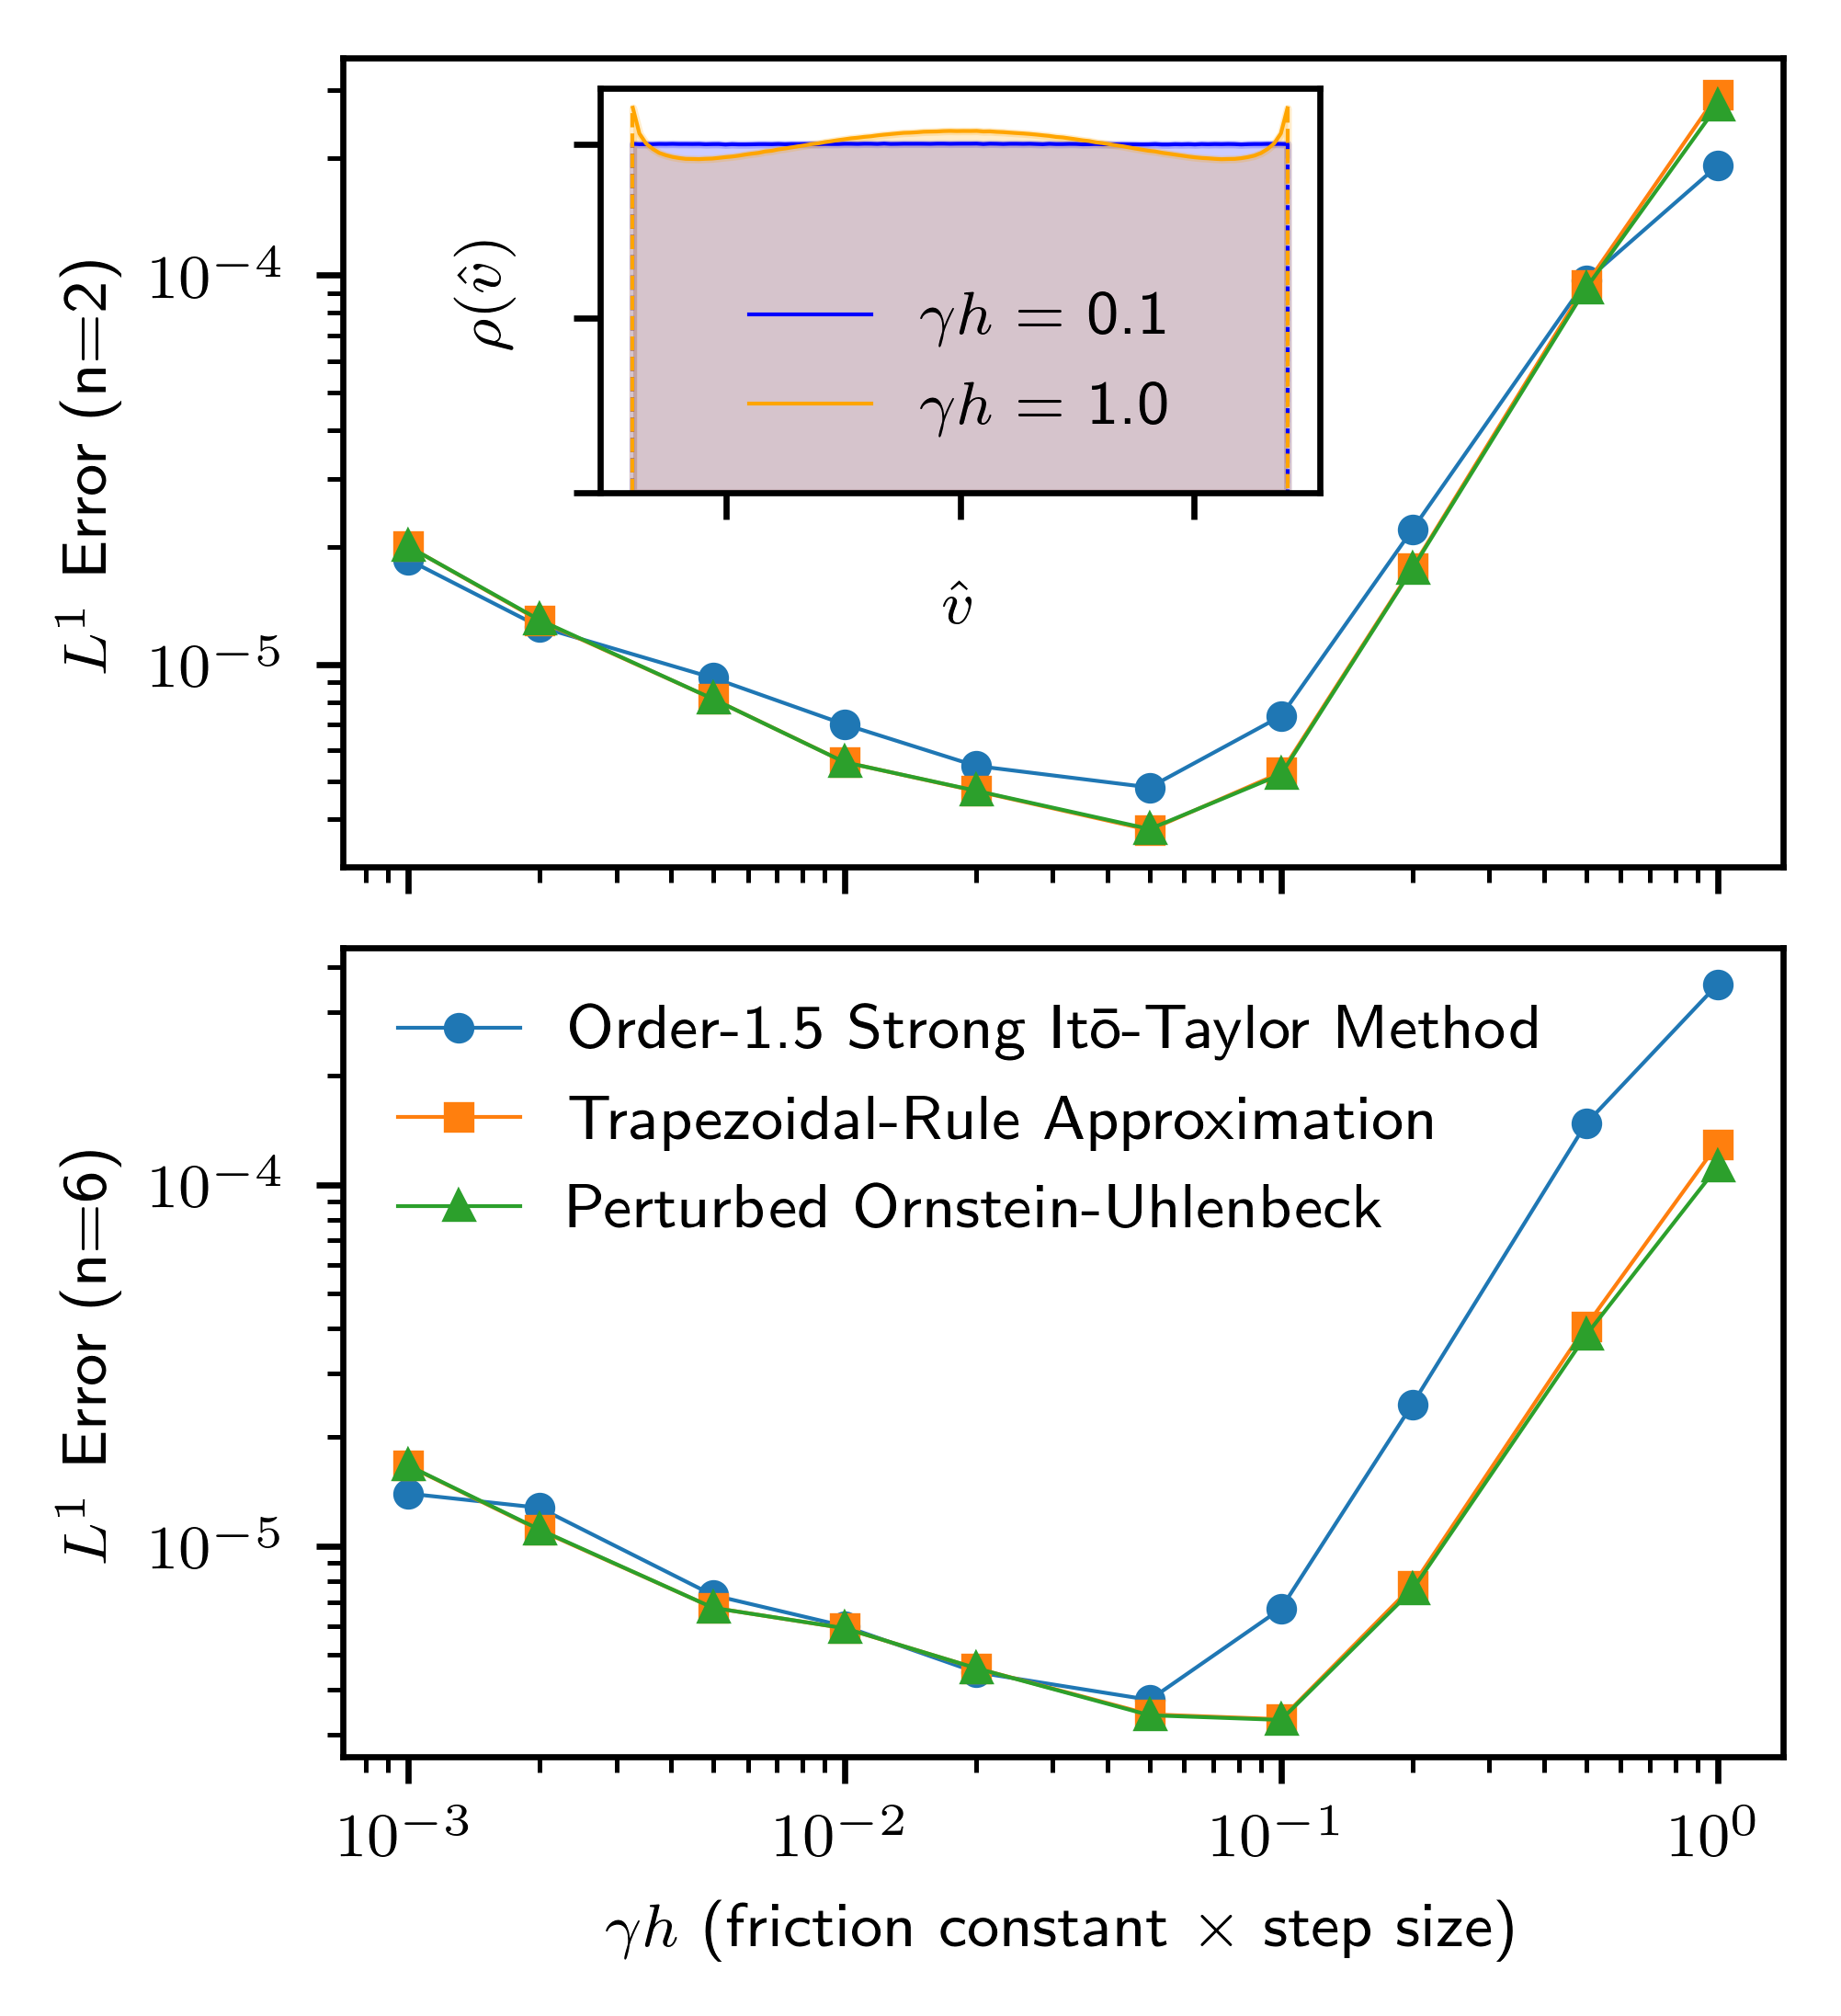
\includegraphics{stochastic_integration}
	\caption{Alternative functions for expressing the momentum dependency of the Hamiltonian.}
	\label{fig:stochastic integration}
\end{figure}

\subsection{Resonance Control in Multiple Time Step Integration of Harmonic Oscillator Dynamics}

\begin{figure}
	\centering
	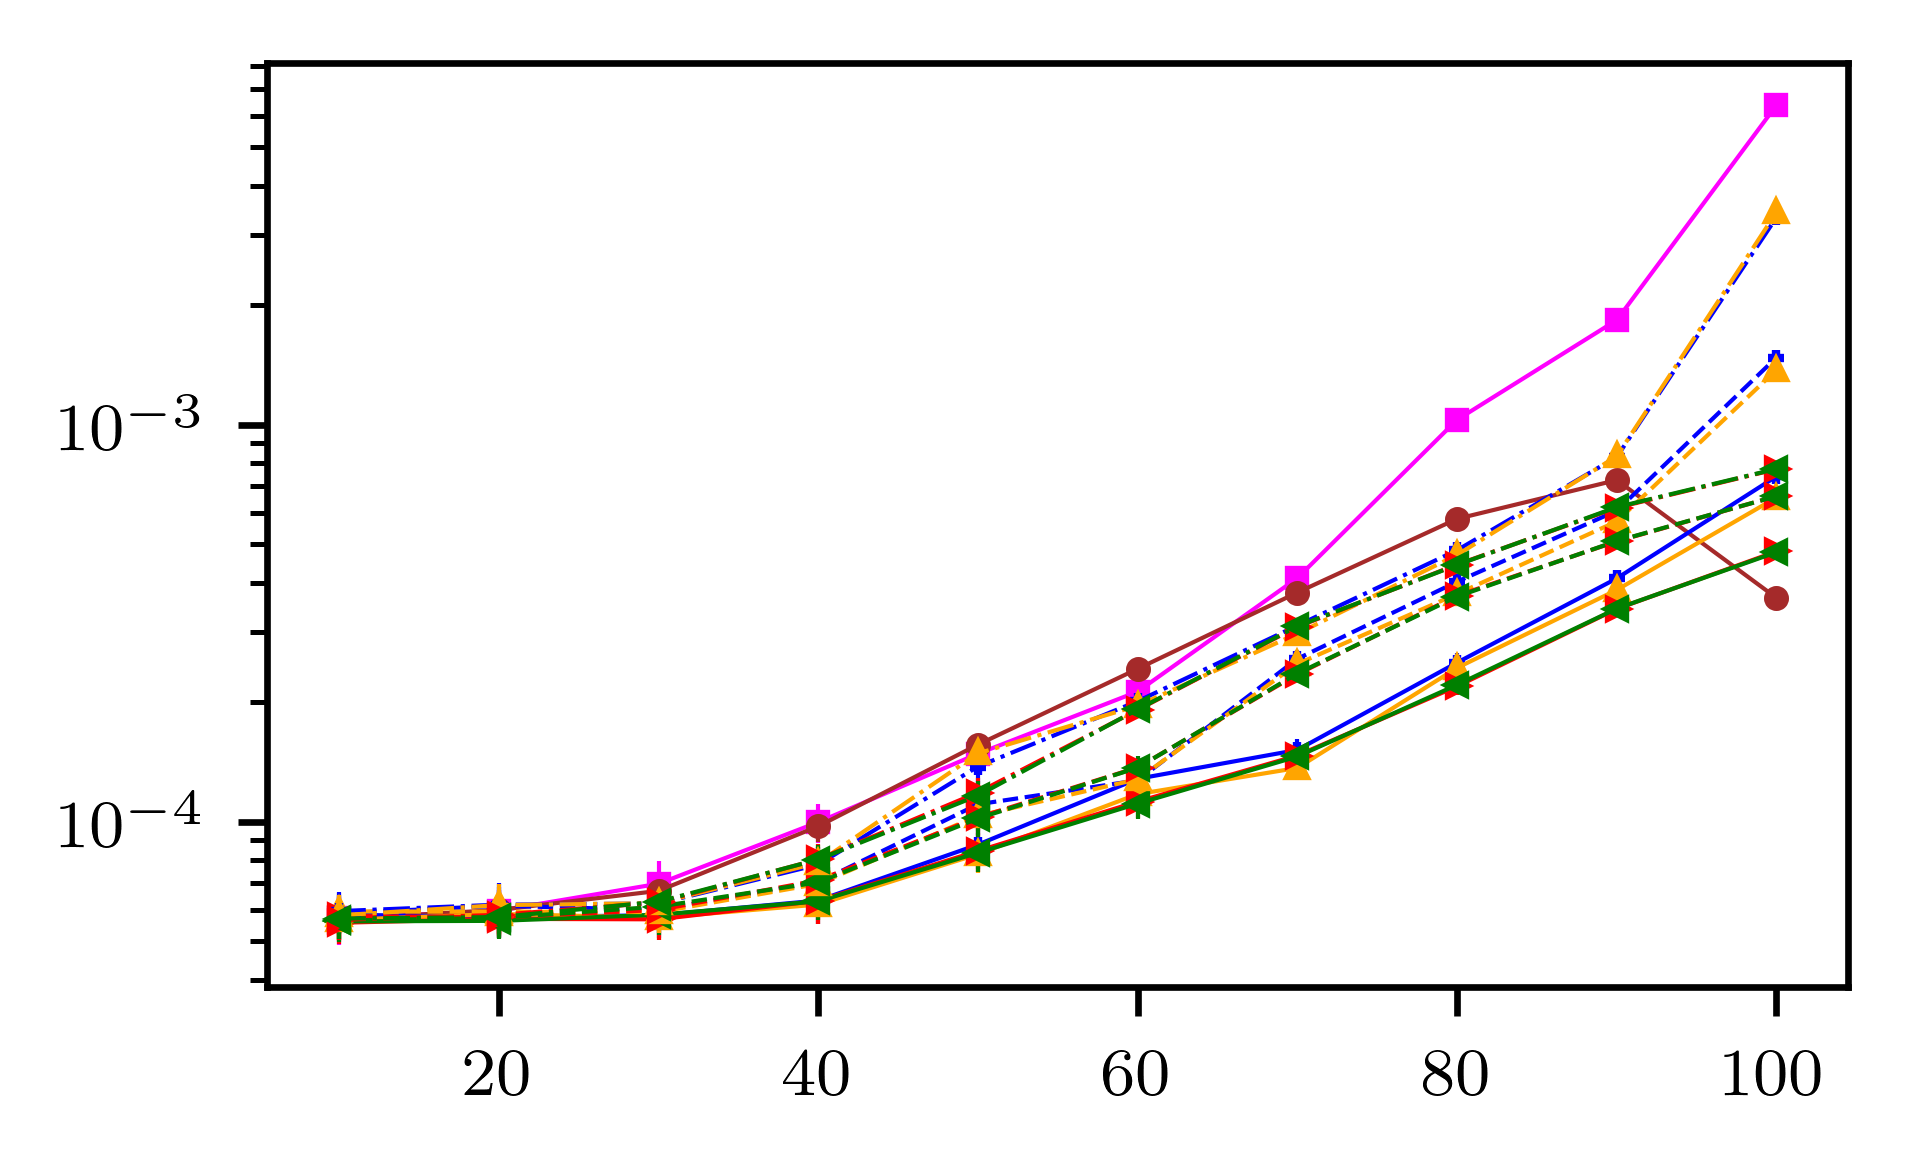
\includegraphics{linear_resonance}
	\caption{Alternative functions for expressing the momentum dependency of the Hamiltonian.}
	\label{fig:linear resonance}
\end{figure}


\subsection{Water}

In order to assess the ability of the new equations of motion to avoid resonance and compare their performance with that of the SIN(R) equations, we have used both methods to run molecular dynamics simulations of liquid water.
For this, we considered $512$ water molecules in a cubic box with side length equal to $24.68~{\rm \AA}$ under periodic boundary conditions.
The simulated temperature was $300~{\rm K}$.
We adopted the parameters of the fully-flexible q-SPC-Fw model \cite{Paesani_2006} and set $r_{\rm cut} = 10~{\rm \AA}$ as the cut-off distance for the Lennard-Jones interactions.
A smoothing 5th-degree spline function was multiplied to the potential energy from $9~{\rm \AA}$ up to cutoff, and no long-distance dispersion correction was used.
The same cut-off distance of $10~{\rm \AA}$ was adopted for the direct-space part of the Ewald-sum, with a damping parameter computed by $\alpha = {\sqrt{-\ln(2\delta)}}/{r_{\rm cut}}$, where $\delta = 1\times10^{-5}$.
The reciprocal-space part was solved using the Particle-Mesh Ewald (PME) method with $n_{\rm mesh} = \frac{2}{3} \alpha L_{\rm box} \delta^{-1/5}$.
Integration was done using the multiple time-scale RESPA algorithm using the RESPA2 scheme described in Ref.~\citenum{Leimkuhler_2013}.
The switch from short- to long-range forces was done in a smooth way from $5~{\rm \AA}$ to $8~{\rm \AA}$ using a 5th-degree spline function again.
However, it is important to remark that, in this case, the smoothing function was applied directly to the forces, rather than to the potential energy.
A friction constant $\gamma = 0.1~{\rm fs}^{-1}$ and a time-scale parameter $\tau = 10~{\rm fs}$ was employed for both the SIN(R) method and for the new equations.
Then, we computed $Q_1 = Q_2 = kT \tau^2$ for SIN(R) and $Q_\eta = L kT \tau^2$ for the new method.
The time-step sizes considered for the shortest and intermediary time scales were $0.5~{\rm fs}$ and $3~{\rm fs}$, respectively, while the step size for the largest time scale varied from $9~{\rm fs}$ to $180~{\rm fs}$.
The total time of every simulation was $3.6~{\rm ns}$, with the last $3~{\rm ns}$ employed to estimate ensemble averages.
Fig.~\ref{fig:liquid water simulation results} contain results obtained for the average potential energy per molecule, as well as for the atomic and  molecular pressures, respectively defined as
\begin{multline}
P_{\rm atom} = \frac{N_{\rm atom} kT + \langle W_{\rm atom} \rangle}{V}
\\ {\rm and} \\
P_{\rm mol} = \frac{N_{\rm mol} kT + \langle W_{\rm mol} \rangle}{V}.
\end{multline}

As one can see in Fig.~\ref{fig:liquid water simulation results}, the two methods exhibit very similar performances.
It is interesting to compare their results with those shown as dashed horizontal lines, which come from a single-time scale integration with a very small time step ($0.2~{\rm fs}$).
Regardless of the method, $L=1$ tends to produce better results than do larger values of $L$.
In all cases, the accuracy of the computed configurational properties decays as the size of the largest time step increases.
Finally, atomic pressure is always very poorly predicted, similarly to what has been observed for other methods using multiple time step integration schemes \cite{Andoh_2017}.
Since this problem does not occur in the same extent for the molecular pressure, we conclude that its origin lies in the handling of intramolecular potential terms.

\begin{figure}
	\centering
	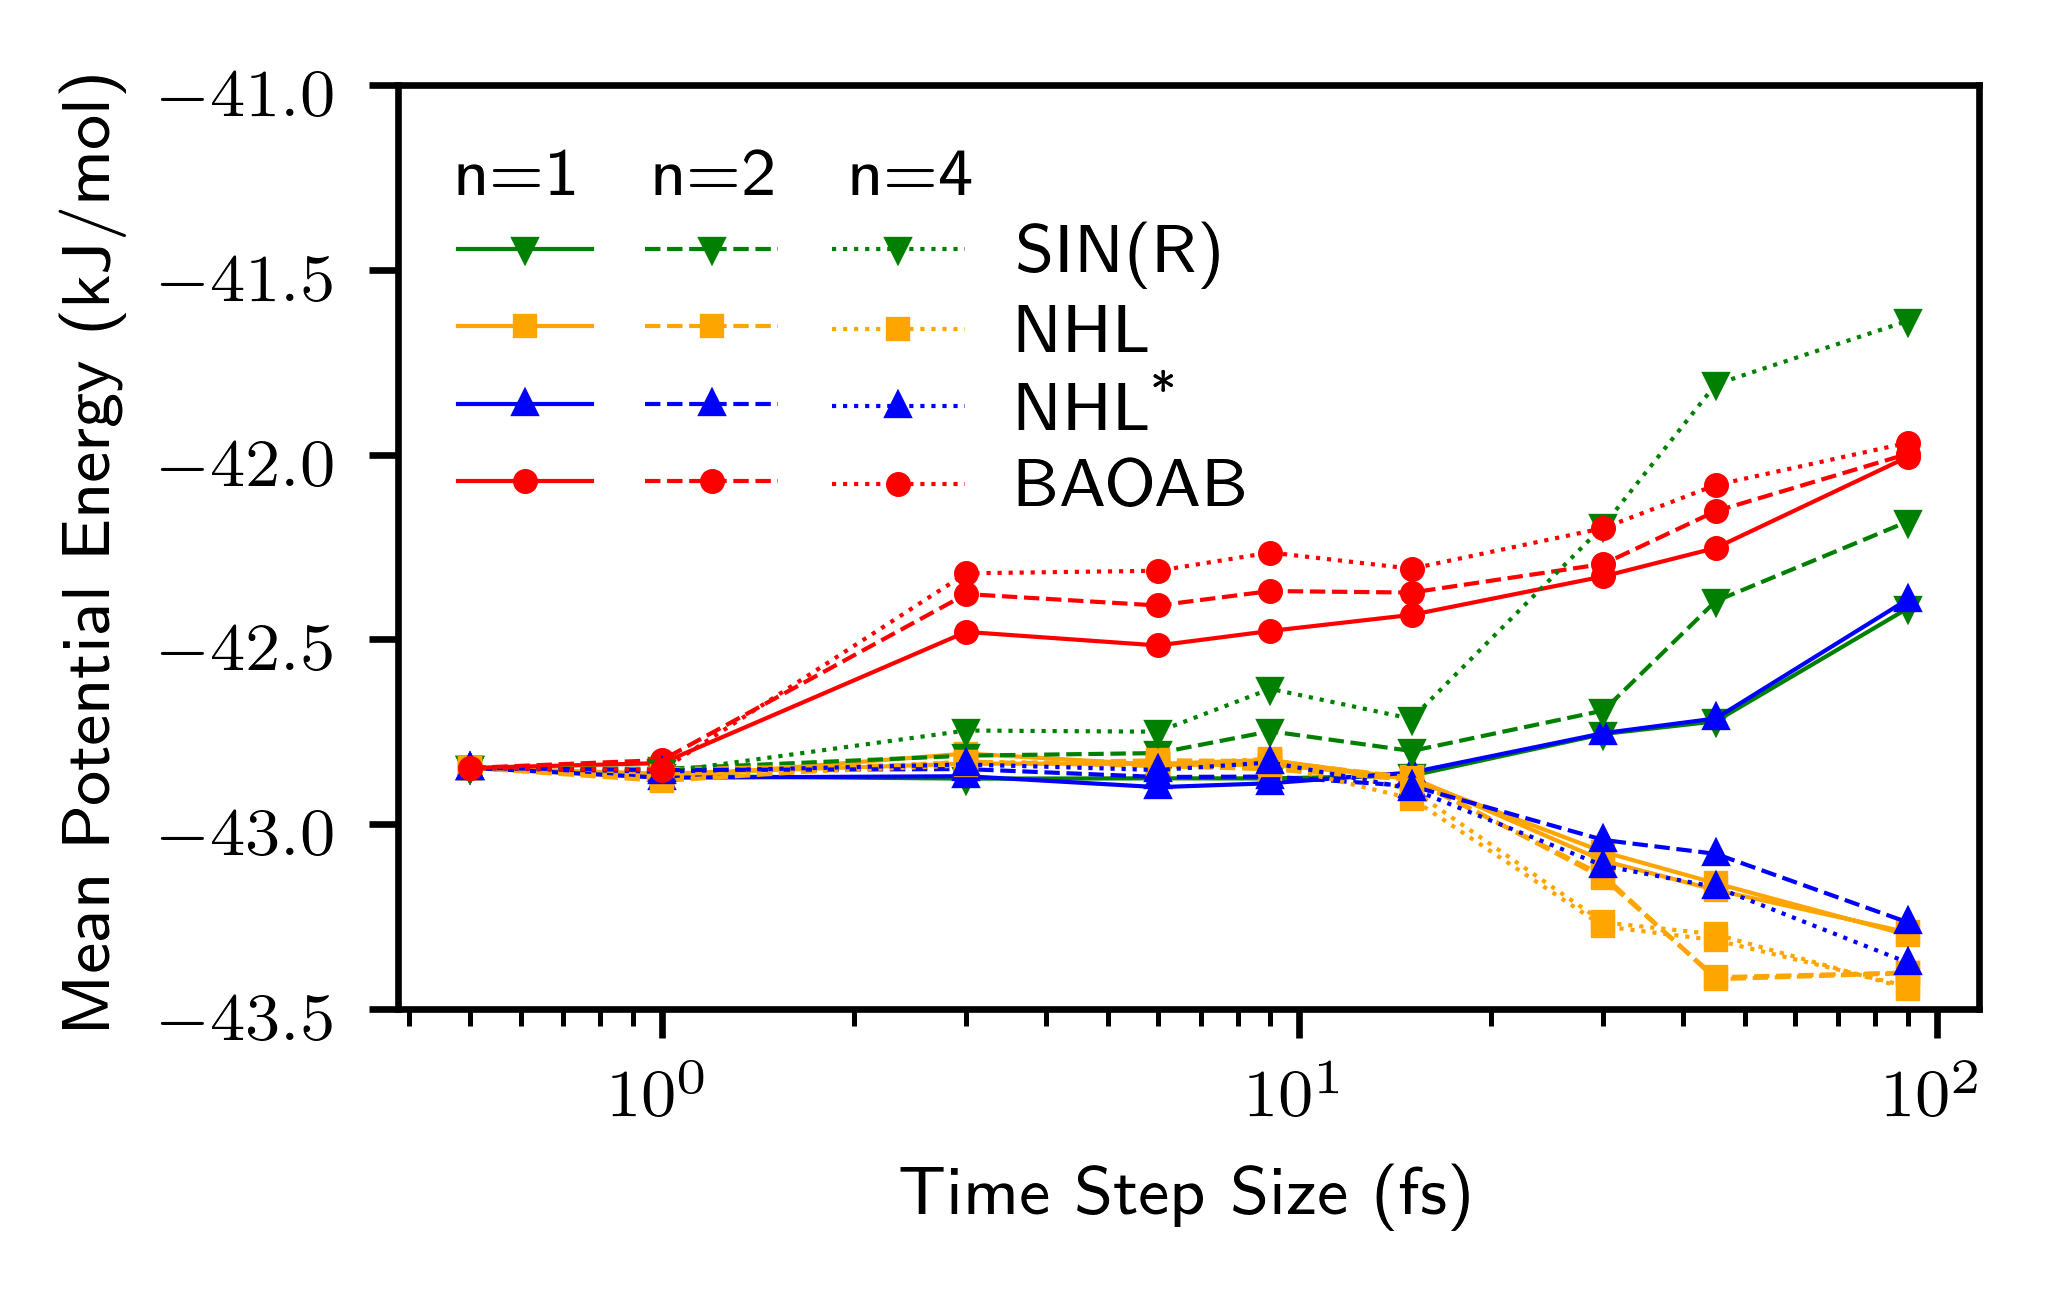
\includegraphics{water_potential_energy}
	\caption{Results obtained from simulations of liquid water using the new equations of motion and the SIN(R) method.}
	\label{fig:liquid water simulation results}
\end{figure}


\section{Conclusion}

\appendix

\section{Momentum and Velocity Distributions in a Canonical Ensemble with the Modified Hamiltonian}
\label{sec:momentum and velocity distributions}

In an NVT ensemble corresponding to the Hamiltonian ${\mathcal H}_n$ defined in Eq.~\eqref{eq:modified hamiltonian}, the probability of each momentum $p_i$ is proportional to $e^{-\nn\ln\cosh(p_i/\sqrt{\nn m_i kT})}$.
This can be represented as
\begin{equation*}
\rho_n(p_i) = \frac{1}{C_n} \sech^\nn\left(\frac{p_i}{\sqrt{\nn m_i k T}}\right),
\end{equation*}
where $C_n$ is a normalization constant.
Because the velocity $v_i$ is a monotonic function of $p_i$, it is straightforward to obtain the velocity probability density $\varrho_n(v_i)$.
Considering that $p_i = f(v_i)$, the relation between the two probability densities is $\varrho_n(v_i) = |f^\prime(v_i)| \rho_n\left(f(v_i)\right)$.
From Eq.~\eqref{eq:velocity definition},
\begin{equation}
\label{eq:momentum as a function of velocity}
f(v_i) = \sqrt{\nn m_i k T}\arctanh\left(\sqrt{\frac{m_i}{\nn k T}} v_i\right).
\end{equation}

%Therefore,
%\begin{equation*}
%\varrho_n(v_i) = \frac{m_i}{\left|1-\frac{m_i v_i^2}{\nn k T}\right|} \frac{1}{C_n} \sech^\nn\left(\arctanh\left(\sqrt{\frac{m_i}{\nn k T}} v_i\right)\right).
%\end{equation*}

Next, the identity $\sech(\arctanh(y)) = \sqrt{1-y^2}$ and the fact that $v_i$ is bounded make
\begin{equation*}
\varrho_n(v_i) = \begin{cases}
\frac{m_i}{C_n} \left(1-\frac{m_i v_i^2}{\nn k T}\right)^{\frac{\nn}{2} - 1} & \mathrm{if} \; v_i^2 \leq \frac{\nn k T}{m_i} \\
0 & \mathrm{otherwise}
\end{cases}.
\end{equation*}

Finally, we can use the fact that $\int_{-\infty}^\infty \varrho_n(v_i) dv_i = 1$ so as to determine an expression for the constant $C_n$.
By changing variables from $v_i$ to $z = \frac{v_i}{\sqrt{{\nn k T}/{m_i}}}$, we obtain
\begin{equation}
\frac{C_n}{\sqrt{\nn m_i k T}} = \int_{-1}^{1} (1-z^2)^{\frac{\nn}{2}-1} dz = \frac{\sqrt{\pi} \Gamma\left(\frac{\nn}{2}\right)}{\Gamma\left(\frac{\nn+1}{2}\right)},
\end{equation}
where $\Gamma(\cdot)$ is the (complete) gamma function.
The same change of variables can be use to evaluate the central moments of the velocity distribution.
Because is is symmetric, all odd-order moments are null, and the even-order ones can be obtained by solving
\begin{equation}
\langle z^{2m} \rangle = \frac{\Gamma\left(\frac{\nn+1}{2}\right)}{\sqrt{\pi} \Gamma\left(\frac{\nn}{2}\right)} \int_{-1}^{1} z^{2m} (1-z^2)^{\frac{\nn}{2}-1} dz,
\end{equation}
where $m$ is a positive integer number.
Then, we obtain the general formula
\begin{equation}
\langle v_i^{2m} \rangle = \frac{\Gamma\left(\frac{\nn+1}{2}\right) \Gamma\left(\frac{2m+1}{2}\right)}{\sqrt{\pi}\Gamma\left(\frac{\nn+2m+1}{2}\right)} \left(\frac{\nn k T}{m_i}\right)^m.
\end{equation}

\section{Metric Determinant and Conservation Law for the Modified NHC Equations}
\label{sec:adapted NHC proofs}

The first goal of this appendix is to prove the validity of Eq.~\eqref{eq:isokinetic NHC metric determinant}, which expresses the metric determinant implied by the modified NHC equations of motion.
As another way of representing it, we can state that $\sqrt{g} = e^{-w(\vt r, \vt v_\eta)}$, where $w$ satisfies Eq.~\eqref{eq:extended space compressibility} \cite{Tuckerman_1999, Tuckerman_2001}.
As stated in Sec.~\ref{sec:massive NHC thermostatting}, the time derivative of $w$ can be evaluated by chain rule as $\dot{w} = \tr{\dot{\vt x}} \diff{\vt x}{w}$.
Therefore, what we must prove here is that \cite{Ezra_2004}
\begin{equation}
\label{eq:metric determinant proof equality}
\tr{\dot{\vt x}} \diff{\vt x}{w} = \nabla_{\vt x} \cdot \dot{\vt x},
\end{equation}
with $w$ compliant with Eq.~\eqref{eq:isokinetic NHC metric determinant} and $\dot{\vt x}$ given by Eq.~\eqref{eq:isokinetic NHC equations}.
After evaluation of the $w$ gradient, the left-hand side above reads
\begin{equation*}
\tr{\dot{\vt x}} \diff{\vt x}{w} = \frac{1}{kT} \sum_{i=1}^{N_f} \left(\dot{r}_i \diff{r_i}{U} + \sum_{j=1}^\nn \dot{v}_{\eta_{j,i}} Q v_{\eta_{j,i}} \right).
\end{equation*}

Next, by substituting the corresponding derivatives from Eq.~\eqref{eq:isokinetic NHC equations}, as well as the definition of force, we obtain
\begin{multline*}
\tr{\dot{\vt x}} \diff{\vt x}{w} = \frac{1}{kT} \sum_{i=1}^{N_f} \Bigg[-F_i v_i \\ 
+ \left(\frac{\nn+1}{\nn} m_i v_i^2 - kT - Q v_{\eta_{2, i}} v_{\eta_{1, i}}\right) v_{\eta_{1,i}} \\
+ \sum_{j=2}^\nn \left(Q v_{\eta_{j-1, i}}^2 - kT - Q v_{\eta_{j+1, i}} v_{\eta_{j, i}}\right) v_{\eta_{j,i}} \Bigg].
\end{multline*}

Many of the terms above cancel out, after which the expression can be simplified to
\begin{multline*}
\tr{\dot{\vt x}} \diff{\vt x}{w} = \sum_{i=1}^{N_f} \bigg[- v_{\eta_{1,i}}\left(1 - \frac{m_i v_i^2}{\nn kT}\right) \\
-\left(F_i - v_{\eta_{1,i}} m_i v_i\right) \frac{v_i}{kT} - \sum_{j=2}^\nn v_{\eta_{j,i}} \bigg].
\end{multline*}

We now turn the attention to the right-hand side of Eq.~\eqref{eq:metric determinant proof equality}, which evaluates in accordance with Eq.~\eqref{eq:isokinetic NHC equations} to
\begin{multline*}
\nabla_{\vt x} \cdot \dot{\vt x} = \sum_{i=1}^{N_f} \left(\diff{p_i}{\dot{p}_i} + \diff{\theta_i}{\dot{\theta}_i} + \sum_{j=1}^{\nn-1} \diff{v_{\eta_{j,i}}}{\dot{v}_{\eta_{j,i}}}\right) = \\
= \sum_{i=1}^{N_f} \Bigg[- v_{\eta_{1,i}} m_i \diff{p_i}{v_i} - \left(F_i - v_{\eta_{1,i}} m_i v_i\right) \frac{v_i}{kT} - \sum_{j=2}^\nn v_{\eta_{j,i}} \Bigg].
\end{multline*}

Hence, after substitution of Eq.~\eqref{eq:velocity derivative wrt momentum}, it becomes evident by comparison that Eq.~\eqref{eq:metric determinant proof equality} holds.

Our second goal is to prove that the property $\Phi_i$, as expressed in Eq.~\eqref{eq:isokinetic NHC conserved quantity}, is an integral of motion (i.e. a conserved quantity) of the modified NHC dynamics.
By applying a logarithm to both sides of Eq.~\eqref{eq:isokinetic NHC conserved quantity} and differentiating the result with respect to time, we get
%Logarithm:
%\begin{equation}
%\ln \Phi_i = \ln \theta_i + \nn \ln \cosh\left(\frac{p_i}{\sqrt{\nn m_i k T}}\right).
%\end{equation}
%
%Taking the time derivative:
\begin{equation}
\frac{d \ln \Phi_i}{dt} = \frac{d \ln \theta_i}{dt} + \sqrt{\frac{\nn}{m_i kT}}  \tanh\left(\frac{p_i}{\sqrt{\nn m_i k T}}\right) \frac{d p_i}{dt}.
\end{equation}

Then, with the aid of Eq.~\eqref{eq:velocity definition}, we can write
\begin{equation}
\frac{\dot{\Phi}_i}{\Phi_i} = \frac{\dot{\theta}_i}{\theta_i} + \frac{v_i \dot{p}_i}{kT}.
\end{equation}

Finally, substitution of $ \dot{p}_i$ and $\dot{\theta}_i$ from Eqs.~\eqref{eq:isokinetic NHC equations p} and \eqref{eq:isokinetic NHC equations theta} leads to the conclusion that $\dot{\Phi}_i = 0$.

\bibliography{modified_hamiltonian}

\end{document}